% magic comments for offline TeX editors:
% !TEX encoding = UTF-8 Unicode
% !TeX TS-program = xelatexmk
% !BIB program = biber

% to display notes, uncomment the following line:
% \setbeameroption{show only notes}
\documentclass[aspectratio=169,19pt,xetex,handout]{beamer}
\usetheme{default}
\usepackage[main=american]{babel}

% bibliography
\usepackage[
backend=biber,
style=alphabetic,
sorting=nyt,
giveninits=true,
maxbibnames=99
]{biblatex}
\addbibresource{dkf-pres.bib}

% standard loads
\graphicspath{ {./graphics/} }
\usepackage{pstricks}

% misc packages
\usepackage{amsmath,amssymb,amsthm,amscd} % maths
\usepackage{dsfont, bbm} % provides \mathds{1}
\usepackage{csquotes}

% load our own fonts; don't use for math
\usefonttheme{professionalfonts} % needed for fontspec with beamer
\usepackage[no-math]{fontspec}
\usepackage[varg,libertine]{newtxmath}

% titles
\newfontfamily\minion{minion-pro}[
Path           = ./minion-font/,
Extension      = .otf,
UprightFont    = *-semibold,
BoldFont       = *-bold,
ItalicFont     = *-semibold-it,
BoldItalicFont = *-bold-italic,
Ligatures      = {Required, Common},
% SmallCapsFeatures={Letters=SmallCaps},
Kerning        = {On},
RawFeature     = {+liga,+salt,+calt,+kern} ]

% main text
\newfontfamily\freight{freight-sans-pro}[
Path           = ./freight-sans-font/,
Extension      = .otf,
UprightFont    = *-book,
BoldFont       = *-bold,
ItalicFont     = *-book-italic,
BoldItalicFont = *-bold-it,
Ligatures      = {Required, Common},
Kerning        = {On},
RawFeature     = {+liga,+salt,+calt,+kern} ]

\setmainfont{minion-pro}[
Path           = ./minion-font/,
Extension      = .otf,
UprightFont    = *-semibold,
BoldFont       = *-bold,
ItalicFont     = *-semibold-it,
BoldItalicFont = *-bold-italic,
Ligatures      = {Required, Common},
Kerning        = {On},
RawFeature     = {+liga,+salt,+calt,+kern}]

\setsansfont{freight-sans-pro}[
Path           = ./freight-sans-font/ ,
Extension      = .otf,
UprightFont    = *-book,
BoldFont       = *-bold,
ItalicFont     = *-book-italic,
BoldItalicFont = *-bold-it,
Ligatures      = {Required, Common},
Kerning        = {On},
RawFeature     = {+liga,+salt,+calt,+kern} ]

% font sizes
% series=\scshape for small caps
\setbeamerfont{title}{size=\Huge,family=\minion,series=\bfseries}
\setbeamerfont{author}{size=\Large,family=\minion}
\setbeamerfont{frametitle}{family=\minion}
\setbeamerfont{normal text}{size=\Large,family=\freight}
\renewcommand*{\bibfont}{\scriptsize}

%%%%%%%%%%%%%%%%%%%%%%%%%%%%%%%%%%%%%%%%%%%%%%%%%
% define colors from Brown U visual identity
\definecolor{red}{HTML}{ED1C24} % "the red"
\definecolor{brown}{HTML}{4E3629} % "Brown's brown"
\definecolor{gold}{HTML}{FFC72C} % "the gold"
\definecolor{gray}{HTML}{98A4AE}
\definecolor{skyblue}{HTML}{59CBE8}
\definecolor{emerald}{HTML}{00B398}
\definecolor{navy}{HTML}{003C71}
\definecolor{taupe}{HTML}{B7B09C}

\definecolor{green}{HTML}{046A38} % "Ivy green"

% use colors
\setbeamercolor*{palette primary}{fg=brown,bg=emerald}
\setbeamercolor*{palette secondary}{fg=brown,bg=emerald}
\setbeamercolor*{palette tertiary}{fg=brown}
\setbeamercolor*{palette quaternary}{fg=brown}

\setbeamercolor{structure}{fg=brown}
\setbeamercolor{author}{fg=brown}

\setbeamercolor{normal text}{fg=brown}
\setbeamercolor{alerted text}{fg=red,bg=brown}
\setbeamercolor{example text}{fg=brown}

\setbeamercolor{block title}{}
\setbeamercolor{block body}{fg=red,bg=brown}

\setbeamercolor{bibliography entry title}{fg=brown} 
\setbeamercolor{bibliography entry location}{fg=navy} 
\setbeamercolor{bibliography entry note}{fg=navy}

\addtobeamertemplate{block begin}{\pgfsetfillopacity{0.75}}{\pgfsetfillopacity{1}}
\addtobeamertemplate{block alerted begin}{\pgfsetfillopacity{0.75}}{\pgfsetfillopacity{1}}
\addtobeamertemplate{block example begin}{\pgfsetfillopacity{0.75}}{\pgfsetfillopacity{1}}

% macros
\DeclareMathOperator{\Prob}{\mathbb{P}}
\DeclareMathOperator{\Exp}{\mathbb{E}}
\DeclareMathOperator{\var}{\mathbb{V}}
\DeclareMathOperator{\cov}{cov}
\DeclareMathOperator*{\sign}{\text{sign}}

\newcommand{\ind}{{\mathds{1}}}
\newcommand{\bs}{\boldsymbol}
\newcommand{\eqd}{\triangleq}
\newcommand{\tr}{\intercal}
\newcommand{\intd}{\mspace{1.5mu}d}

\newcommand{\dataset}{{\cal D}}
\newcommand{\fracpartial}[2]{\frac{\partial #1}{\partial  #2}}
\newcommand{\N}{\ensuremath{\mathcal{N}}}
\newcommand{\RR}{\ensuremath{\mathbb{R}}}
\DeclareMathOperator*{\argmax}{\arg\max}
\DeclareMathOperator*{\argmin}{\arg\min}
\DeclareMathOperator{\tv}{tv}
\renewcommand{\SS}{\ensuremath{\mathbb{S}}}

\newcommand{\eqrefMT}[1]{(\ref{#1})}
\renewcommand{\eqref}[1]{eq.~\eqrefMT{#1}}
\newcommand{\eqrefs}[1]{Eqs.~\eqrefMT{#1}}
\newcommand{\Eqref}[1]{Eq.~\eqrefMT{#1}}
\newcommand{\Eqrefs}[1]{Eqs.~\eqrefMT{#1}}

\newtheorem{assumption}{Assumption}
\newtheorem{thm}{Theorem}

\providecommand{\abs}[1]{\ensuremath{\left\lvert#1\right\rvert}}
\providecommand{\norm}[1]{\ensuremath{\left\lVert#1\right\rVert}}

\newtheorem{proposition}[theorem]{Proposition} 
\newtheorem{remark}[theorem]{Remark}
\newtheorem{axiom}[theorem]{Axiom}

% drawing bayes nets
\usepackage{tikz}
\usetikzlibrary{bayesnet,overlay-beamer-styles,matrix}
\tikzset{>=latex}

\usepackage{tikz-cd}
\usetikzlibrary{cd,patterns,decorations.pathmorphing,decorations.pathreplacing}

% specs for xcolor's fcolorbox
\fboxsep=1pt % padding thickness
\fboxrule=1pt % border thickness

% background canvas
\setbeamertemplate{background canvas}{%
\begin{tikzpicture}[remember picture,overlay]
\shade[left color=skyblue,right color=taupe]
  (current page.north west)
     rectangle
  (current page.south east);
\end{tikzpicture}%
}

\setbeamertemplate{background}{%
    
\includegraphics[width=\paperwidth,height=\paperheight,keepaspectratio]{brownlogo}}

% no nav symbols
\setbeamertemplate{navigation symbols}{}
\setbeamertemplate{footline}{}
\renewcommand\footnoterule{}
\renewcommand\thefootnote{}

% no figure labels
\setbeamertemplate{caption}{\raggedright\insertcaption\par}

% numbered sections in toc
\setbeamertemplate{section in toc}[sections numbered]

% Rhode Island level -> over 9000
\setbeamertemplate{itemize item}{
\includegraphics[height=8pt]{ri_anchor-brown}}
\setbeamertemplate{itemize subitem}{\raisebox{1pt}{
\includegraphics[height=4pt]{ri_anchor-brown}}}
\setbeamertemplate{bibliography item}{\raisebox{-.5pt}{
\includegraphics[height=6pt]{ri_anchor-brown}}}

% fix all that ugly space between bib item and entry
\defbibenvironment{bibliography}
  {\list{}
     {\settowidth{\labelwidth}{\usebeamertemplate{bibliography item}}%
      \setlength{\leftmargin}{\labelwidth}%
      \setlength{\labelsep}{0.75\biblabelsep}%
      \addtolength{\leftmargin}{\labelsep}%
      \setlength{\itemsep}{\bibitemsep}%
      \setlength{\parsep}{\bibparsep}}}
  {\endlist}
  {\item}

\renewcommand{\bot}{\llcorner\!\!\lrcorner} % vector bottom
\renewcommand{\top}{\ulcorner\!\!\urcorner} % vector top

%%%%%%%%%%%%%%%%%%%%%%%%%%%%%%%%%%%%%%%%%%%%%%%%%
\title[Discriminative Filtering]{\Huge\textbf{A Discriminative Approach to Bayesian Filtering with Applications to Human Neural Decoding}}
\author[M. C. Burkhart]{\Large Michael C. Burkhart}
\institute{Division of Applied Mathematics\\ Brown University\\ Providence, Rhode Island}
\date{23 May 2018}

\begin{document}

%%%%%%%%%%%%%%%%%%%%%%%%%%%%%%%%%%%%%%%%%%%%%%%%%
\frame{\titlepage}
%%%%%%%%%%%%%%%%%%%%%%%%%%%%%%%%%%%%%%%%%%%%%%%%%

\setbeamertemplate{background}{}

\begin{frame}{Overview}
\LARGE
\begin{enumerate}
    \item Bayesian Filtering
    \begin{itemize}
        \item problem description
        \item main approaches
        \item applications
    \end{itemize}
    \medskip
    \item Challenges to Effective Neural Decoding
    \begin{itemize}
        \item what makes this problem hard / unique
        \item drawbacks to current approaches
        \item our solution: the DKF
    \end{itemize}
    \medskip
    \item Nonstationarities
    \begin{itemize}
        \item the problem and proposed solutions
        \item our approach
    \end{itemize}
\end{enumerate}
\end{frame}


%%%%%%%%%%%%%%%%%%%%%%%%%%%%%%%%%%%%%%%%%%%%%%%%%
\section{Bayesian Filtering}
%%%%%%%%%%%%%%%%%%%%%%%%%%%%%%%%%%%%%%%%%%%%%%%%%
\begin{frame}{State-Space Models}
\Large
Consider the following graphical model:
\[
\begin{tikzcd}[ampersand replacement=\&,column sep=large, /tikz/column 5/.append style={anchor=base west}]
Z_1 \arrow[r] \arrow[d]
	\& \cdots \arrow[r]
		\& Z_{t-1} \arrow[r]  \arrow[d]
			\& Z_t \arrow[d] 
			\&{\}\text{ hidden}}\\
	X_1
	\& 
		\& X_{t-1} 
			\& X_t
			    \&{\}\text{ observed}}
\end{tikzcd}
\]

\bigskip

\emph{Filtering} calculates our best guess for $Z_t$ given the sequence of observations $X_1,\dotsc,X_t$.

\note[item]{There is a discrete stochastic process $Z_1,Z_2,\dotsc,Z_t$ about which we are very interested}
\note[item]{At each time step we obtain a measurement $X_t$ related to $Z_t$}

\end{frame}


%%%%%%%%%%%%%%%%%%%%%%%%%%%%%%%%%%%%%%%%%%%%%%%%%
\begin{frame}{Bayesian Filtering}
\Large
In the \emph{Bayesian} approach to filtering, we place a joint distribution on these quantities:
\begin{itemize}
\item The \emph{\textcolor{navy}{state model}} $\textcolor{navy}{p(z_t|z_{t-1})}$ relates the current and previous hidden states.
\item The \emph{\textcolor{green}{measurement model}} $\textcolor{green}{p(x_t|z_t)}$ relates the current observation and hidden state.
\end{itemize}
\[
\begin{tikzcd}[ampersand replacement=\&,column sep=large, /tikz/column 5/.append style={anchor=base west}]
Z_1 \arrow[r,"p(z_2|z_1)" navy] \arrow[d,"p(x_1|z_1)" green]
	\& \cdots \arrow[r,"p(z_{t-1}|z_{t-2})" navy]
		\& Z_{t-1} \arrow[r,"p(z_t|z_{t-1})" navy]  \arrow[d,"p(x_{t-1}|z_{t-1})" green]
			\& Z_t \arrow[d,"p(x_t|z_t)" green] \\
	X_1
	\& 
		\& X_{t-1} 
			\& X_t
\end{tikzcd}
\]
\end{frame}


%%%%%%%%%%%%%%%%%%%%%%%%%%%%%%%%%%%%%%%%%%%%%%%%%
\begin{frame}{The Posterior}
\Large

We are interested in the posterior $\textcolor{red}{p(z_t|x_{1:t})}$.
\note{The posterior is the distributional solution to the filtering problem.}

\bigskip


This can be calculated recursively via:
\[
{\textcolor{red}{p(z_t|x_{1:t})}} \propto \underbrace{{\textcolor{green}{p(x_t|z_t)}} \underbrace{\int {\textcolor{navy}{p(z_t|z_{t-1})}}\; {\textcolor{red}{p(z_{t-1}|x_{1:t-1})}} \; dz_{t-1}}_{\text{ \textcolor{navy}{state update}, gives }p(z_t|x_{1:t-1})}}_{\text{ \textcolor{green}{measurement update}, gives }p(x_t,z_t|x_{1:t-1})}
\]

The proportionality entails dividing by $p(x_t|x_{1:t-1})$.

\end{frame}

%%%%%%%%%%%%%%%%%%%%%%%%%%%%%%%%%%%%%%%%%%%%%%%%%
\begin{frame}{Methodology}
\Large
Approaches to Bayesian filtering mirror approaches to integration:
\note{How do we integrate?
Even your first definitions of integration allude to the many ways we can calculate this\dots originally as the limit of a sum (Riemannian integral), and then for $f\ge 0$ as the supremum of integrals over simple functions $0\leq \phi \leq f$.  Fundamental to the Bayesian approach is the set of tools developed to perform inference (i.e. solve an integral), as follows:}
\onslide<2>{
\begin{itemize}
    \item \textbf{exact}: the Kalman filter~\cite{Kal60,Kal61}, extended by \textcite{Ben81} and \textcite{Dau84,Dau86}
    \item \textbf{variational inference}: Extended Kalman Filter (EKF), Laplace approximation, Gaussian Assumed Density Filter
    \note[item]{variational inference: integration -> optimization}
    \item \textbf{quadrature}: Unscented Kalman Filter~\cite{Jul97}, sigma-point filters~\cite{Wan00,van04}, Cubature and Quadrature Kalman filters~\cite{Ito00,Ara07}
    \note[item]{quadrature: integration -> summation}
    \item \textbf{Monte Carlo}: particle filter, Sequential Importance Sampling~\cite{Ham54} and Resampling~\cite{Gor93}, ensemble Kalman filter~\cite{Ell94}
    \note[item]{MC: integration -> sampling/summation}
\end{itemize}
}
\end{frame}

%%%%%%%%%%%%%%%%%%%%%%%%%%%%%%%%%%%%%%%%%%%%%%%%%
\begin{frame}{Kalman Filter}
\Large
The Kalman filter specifies both the \textcolor{navy}{state model} and \textcolor{green}{measurement model} as linear, Gaussian.
\[
\begin{tikzcd}[ampersand replacement=\&,column sep=2cm, /tikz/column 5/.append style={anchor=base west}]
\textcolor{brown}{Z_{t-1}|X_{1:t-1} }\arrow[r,"\textcolor{navy}{\eta_d(z_t;Az_{t-1},\Gamma)}"] 
	\& Z_t \arrow[d,"\textcolor{green}{\eta_n(x_t;Hz_t,\Lambda)}"] \\
	\& X_t
\end{tikzcd}
\]
If $\textcolor{red}{Z_{t-1}|X_{1:t-1}}\sim \textcolor{red}{\N(\nu_{t-1},\Phi_{t-1})}$
% $\textcolor{red}{p(z_{t-1}|x_{1:t-1})} \propto {\textcolor{red}{\eta_d(z_{t-1};\nu_{t-1},\Phi_{t-1})}}$ 
then
\[
\textcolor{red}{Z_t|X_{1:t}}\sim \textcolor{red}{\N\big(\Phi_t(H ^\intercal \Lambda^{-1}x_t+\hat\Phi_{t-1}^{-1}\hat\nu_{t-1}), \Phi_t \big)}.
\]
\emph{Integration is accomplished with matrix multiplication.}
% \textcolor{red}{p(z_t|x_{1:t})} \propto \textcolor{red}{\eta_d\big(z_t; \Phi_t(H ^\intercal \Lambda^{-1}x_t+\hat\Phi_{t-1}^{-1}\hat\nu_{t-1}), \Phi_t \big)}
\footnotetext{\emph{N.B.}: $\hat \nu_{t-1} = A\nu_{t-1}$, $\hat \Phi_{t-1} = A\Phi_{t-1}A^\intercal + \Gamma$, and 
$\Phi_t = (H^\intercal \Lambda^{-1}H + \hat\Phi_{t-1}^{-1})^{-1}$.}
\end{frame}

%%%%%%%%%%%%%%%%%%%%%%%%%%%%%%%%%%%%%%%%%%%%%%%%%
\setbeamertemplate{background}{%
    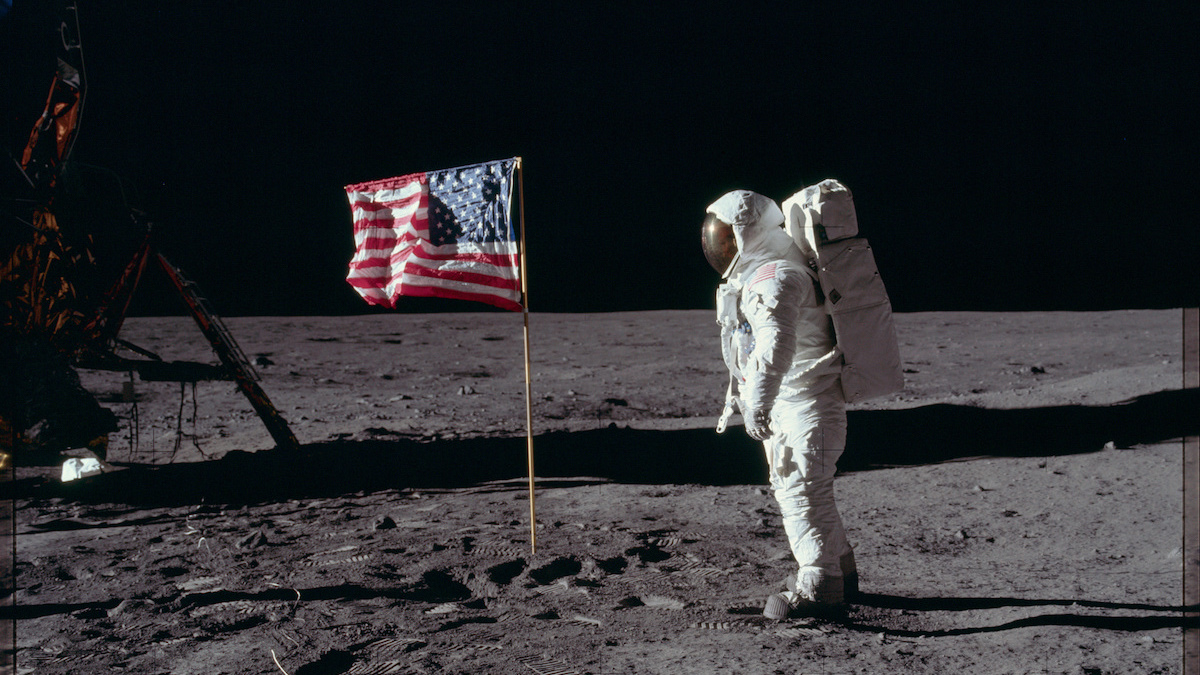
\includegraphics[width=\paperwidth,height=\paperheight,keepaspectratio]{apollo_landing}}
\setbeamercolor{block body}{fg=red,bg=black}

\begin{frame}[t]{}

\vspace{-24pt}
\begin{block}{}
\Large
The Apollo Lunar Module used a variant of the Kalman Filter to land my fellow Purdue grad on the moon~\cite{Hal66,Hoa69,Bat70}.
\end{block}

\footnotetext{\color{red}image credit: N. Armstrong}

\end{frame}

%%%%%%%%%%%%%%%%%%%%%%%%%%%%%%%%%%%%%%%%%%%%%%%%%
\setbeamertemplate{background}{%
    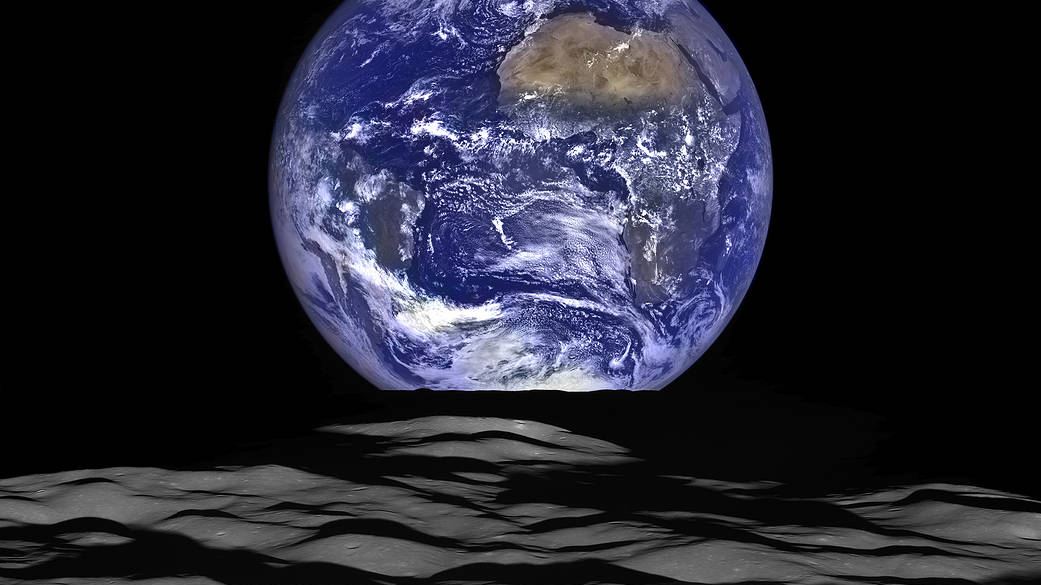
\includegraphics[width=\paperwidth,height=\paperheight,keepaspectratio]{earth_rise}}
\setbeamercolor{block body}{fg=red,bg=gray}

\begin{frame}[b]{}

\begin{block}{}
\Large
GPS receivers use the Extended Kalman filter to model and mitigate satellite clock offset and atmospheric delays~\cite{Axe95,Hof01}.
\end{block}

\footnotetext{\color{red}image credit: NASA}
\end{frame}

%%%%%%%%%%%%%%%%%%%%%%%%%%%%%%%%%%%%%%%%%%%%%%%%%
\setbeamertemplate{background}{%
    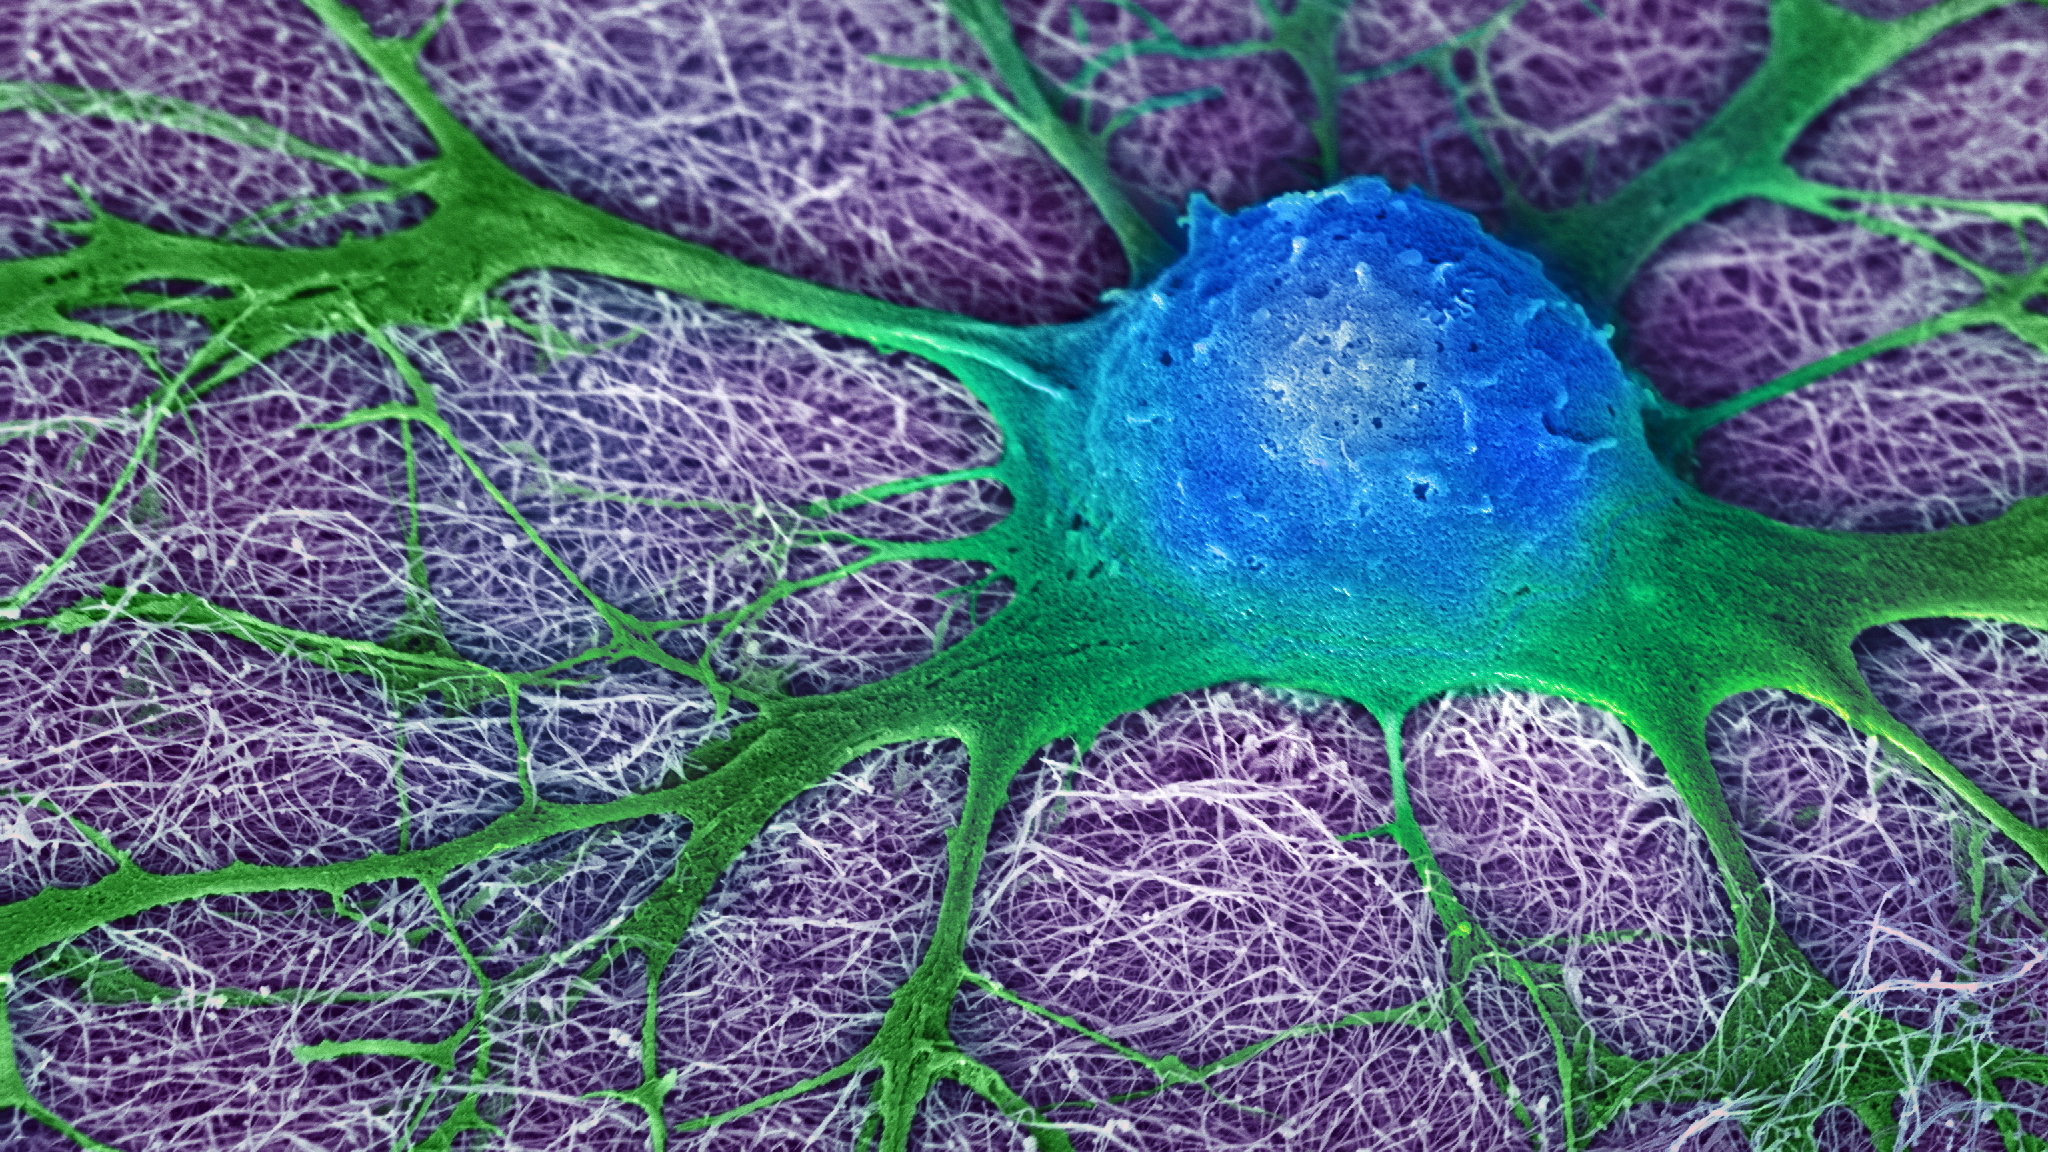
\includegraphics[width=\paperwidth,height=\paperheight,keepaspectratio]{nih_its_alive}}
\setbeamercolor{block body}{fg=brown,bg=skyblue}

\begin{frame}[b]{}

\begin{columns}
\column[t]{.58\textwidth}
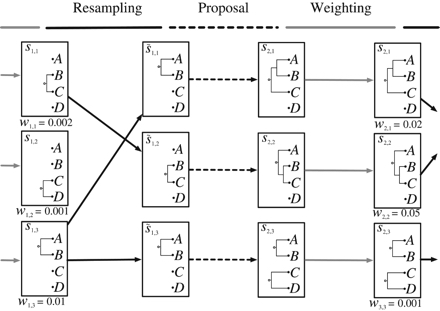
\includegraphics[width=0.7\textwidth]{smc_phylo}
\column{.38\textwidth}
\begin{block}{}
\Large
Sequential Monte Carlo is used to estimate phylogenetic trees~\cite{Bou12,Wan15,Din18}.
\end{block}
\end{columns}

\footnotetext{\pgfsetfillopacity{0.75}\colorbox{skyblue}{\color{black} image credit: NIH; phylogenetics diagram  from~\cite{Bou12}}}
\end{frame}

%%%%%%%%%%%%%%%%%%%%%%%%%%%%%%%%%%%%%%%%%%%%%%%%%
\setbeamertemplate{background}{%
    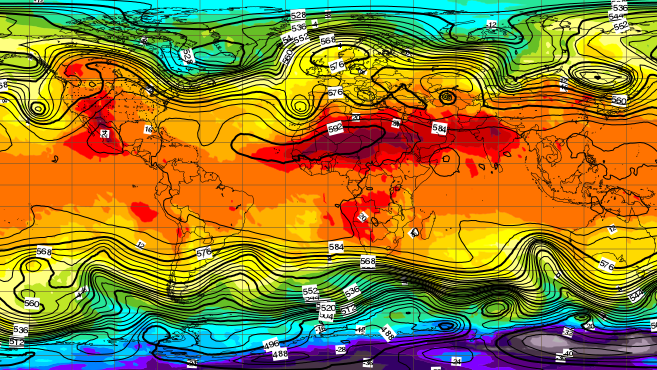
\includegraphics[width=\paperwidth,height=\paperheight,keepaspectratio]{ecmwf-ensemble}}
\setbeamercolor{block body}{fg=brown,bg=taupe}

\begin{frame}[b]{}

\begin{columns}
\column[t]{.38\textwidth}
\column{.58\textwidth}
\begin{block}{}
\Large
\color{black} Weather forecasts assimilate data with ensemble versions of the Kalman filter~\cite{Gei94,Bis01,Ott04,Hun07,Bue17}.
\end{block}
\end{columns}

\footnotetext{\pgfsetfillopacity{0.75}\colorbox{taupe}{\color{black}image credit: European Centre for Medium-Range Weather Forecasts}}
\end{frame}

\setbeamertemplate{background}{}

%%%%%%%%%%%%%%%%%%%%%%%%%%%%%%%%%%%%%%%%%%%%%%%%%
\section{Challenges to Effective Neural Decoding}
%%%%%%%%%%%%%%%%%%%%%%%%%%%%%%%%%%%%%%%%%%%%%%%%%

% \setbeamertemplate{background}{%
%     \includegraphics[width=\paperwidth,height=\paperheight,keepaspectratio]{bibslogo}}
\begin{frame}{General Challenges to Filtering}
\Large
\begin{itemize}
    \item The approximations made by these filters can be quite poor.
    \begin{itemize}
        \item The linear specification of the Kalman filter is very restrictive.
        \item The EKF (that linearizes a nonlinear model) depends on its linearization.
        \item Better approximations tend to require more computational time/resources.
    \end{itemize}
    \medskip
    \item Implementing any of these filters \emph{requires a generative probabilistic model of the process.}
        \begin{itemize}
        \item A filter will only be as good as the model it is given.
        \item Filtering approaches take the model as an input: they provide no guidance on how to learn that model.
    \end{itemize}
\end{itemize}
\end{frame}
% \setbeamertemplate{background}{}

% while they may appear different, 
% the problems we have tacked with filtering
% have a lot of commonalities

%%%%%%%%%%%%%%%%%%%%%%%%%%%%%%%%%%%%%%%%%%%%%%%%%
\begin{frame}{Application: Neural Filtering}

\begin{columns}
\column{0.49\textwidth}
\raggedleft Filter updates need to be calculated in under 20ms.
\column{0.49\textwidth}
\begin{figure}
    \raggedright
    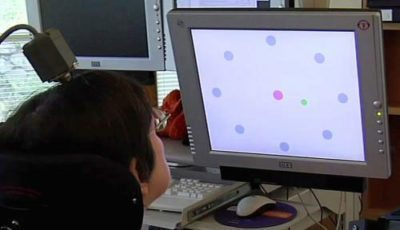
\includegraphics[width=0.9\textwidth]{bg_setup_2}
\end{figure}
\end{columns}

\begin{columns}
\column{0.49\textwidth}
\begin{figure}[t]
    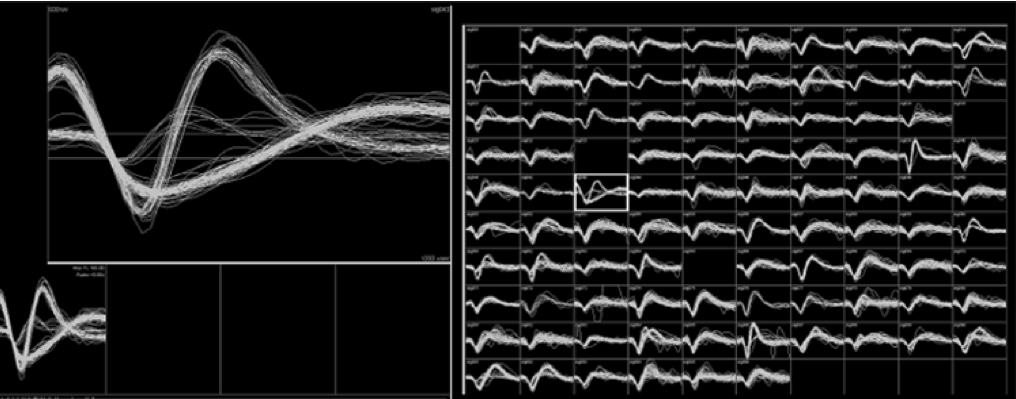
\includegraphics[width=0.9\textwidth]{waveforms}
        \raggedleft
\end{figure}
\column{0.49\textwidth}
\raggedright
The relationship between observations and latent states can be nonlinear.  Observations are very high-dimensional.
\end{columns}

\footnotetext{image credit:~\cite{Sun05}}
\end{frame}

%%%%%%%%%%%%%%%%%%%%%%%%%%%%%%%%%%%%%%%%%%%%%%%%%
\begin{frame}{The Learning Problem}
\Large
Generative approaches to filtering require a model for $p(x_t|z_t)$ \ldots
\begin{figure}
  \begin{tikzpicture}[auto]
    % pictures
    \node (xt) {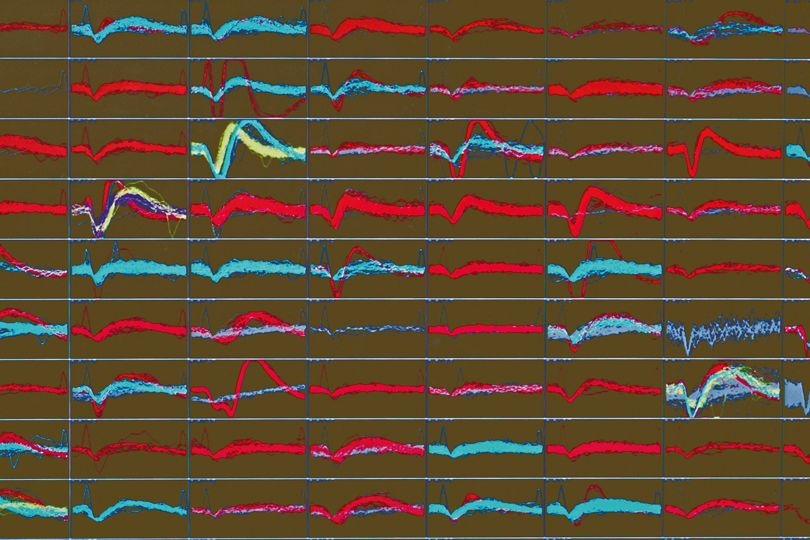
\includegraphics[width=0.4\textwidth]{braingate5}};
    \node (zt) [right=0.2\textwidth of xt]  {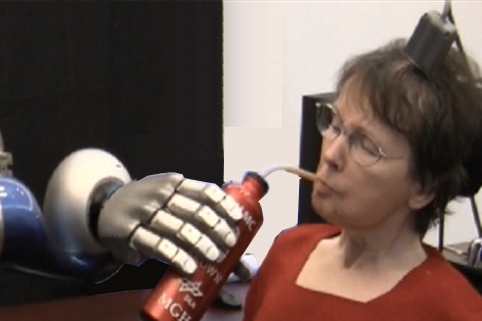
\includegraphics[width=0.4\textwidth]{braingate1}};
    
    % labels
    \node (xlabel) [below=0.01\textwidth of xt] {$X_t$, neural signals in $\RR^{100}$};
    \node (xlabel) [below=0.01\textwidth of zt] {$Z_t$, intentions in $\RR^{3}$};
    
    % edges
    \draw [->,ultra thick,green] (zt) to[bend right] node[midway] {$\textcolor{green}{p(x_t|z_t)}$} (xt);
    \onslide<2->{\draw [->,ultra thick,green] (xt) to[bend right] node[midway] {$\textcolor{green}{p(z_t|x_t)}$} (zt);}
  \end{tikzpicture}
\end{figure}
\onslide<2->{\ldots but what if we could better model $p(z_t|x_t)$?}

\footnotetext{image credit: BrainGate}
\end{frame}

%%%%%%%%%%%%%%%%%%%%%%%%%%%%%%%%%%%%%%%%%%%%%%%%%
\begin{frame}{Discriminative Approach}
\Large
We apply Bayes' rule:
\begin{align*}
{\textcolor{red}{p(z_t|x_{1:t})}} 
\propto & \underbrace{{\textcolor{green}{p(x_t|z_t)}}}_{\Bigg\downarrow} \int {\textcolor{navy}{p(z_t|z_{t-1})}}\; {\textcolor{red}{p(z_{t-1}|x_{1:t-1})} \; dz_{t-1}} \\
\propto & \overbrace{{\textcolor{green}{\frac{p(z_t|x_t)}{p(z_t)}}}}^{} \int {\textcolor{navy}{p(z_t|z_{t-1})}}\; {\textcolor{red}{p(z_{t-1}|x_{1:t-1})} \; dz_{t-1}}
\end{align*}

\end{frame}

%%%%%%%%%%%%%%%%%%%%%%%%%%%%%%%%%%%%%%%%%%%%%%%%%
\begin{frame}{Discriminative Kalman Filter (DKF)}
\Large
The DKF retains a linear, Gaussian \textcolor{navy}{state model}, but takes $\textcolor{green}{p(z_t|x_t)}\propto \textcolor{green}{\tfrac{p(z_t|x_t)}{p(z_t)}}$  and approximates $\textcolor{green}{p(z_t|x_t) \approx \eta_d(z_t;f(x_t),Q(x_t))}$.
\[
\begin{tikzcd}[ampersand replacement=\&,column sep=2cm, /tikz/column 5/.append style={anchor=base west}]
\textcolor{brown}{Z_{t-1}|X_{1:t-1} }\arrow[r,"\textcolor{navy}{\eta_d(z_t;Az_{t-1},\Gamma)}"] 
	\& Z_t \arrow[d," \textcolor{green}{\approx\tfrac{\eta_d(z_t;f(x_t),Q(x_t))}{\eta_d(z_t;0,S)}}"] \\
	\& X_t
\end{tikzcd}
\]
If $\textcolor{red}{Z_{t-1}|X_{1:t-1}}\sim \textcolor{red}{\N(\mu_{t-1},\Sigma_{t-1})}$
% $\textcolor{red}{p(z_{t-1}|x_{1:t-1})} \propto {\textcolor{red}{\eta_d(z_{t-1};\mu_{t-1},\Sigma_{t-1})}}$ 
then
\[
\textcolor{red}{Z_{t}|X_{1:t}}\sim \textcolor{red}{\N(\mu_t,\Sigma_t)}
\]
% \textcolor{red}{p(z_t|x_{1:t})} \propto \textcolor{red}{\eta_d\big(z_t; \mu_t, \Sigma_t \big)}
\emph{The DKF: a nonlinear relationship between $Z_t$ and $X_t$ with closed-form updates.} 
\footnotetext{\emph{N.B.}: $M_t = A\Sigma_{t-1}A^\tr+\Gamma$, 
$\Sigma_t  = (Q(x_t)^{-1}+M_t^{-1}-S^{-1})^{-1}$, and 
$\mu_t  = \Sigma_t(Q(x_t)^{-1}f(x_t) + M_t^{-1}A\mu_{t-1})$ for $(Q(x_t)^{-1}-S^{-1})^{-1}$ pos.-definite.}
\end{frame}

%%%%%%%%%%%%%%%%%%%%%%%%%%%%%%%%%%%%%%%%%%%%%%%%%
\begin{frame}{Normality \& the Bayesian CLT}
For $\Theta\sim\operatorname{Uniform}([0,1])$, draw a sequence:
\[
X_1, X_2 \dotsc\sim^\text{i.i.d.}\operatorname{Bernoulli}(\Theta)
\]
Then:
\[
p(\theta | x_1,\dotsc, x_n)
 \propto \theta^{n\bar x} (1-\theta)^{n(1-\bar x) } \mathds{1}_{[0,1]}(\theta)
\]
where $\bar x =  \tfrac{1}{n}\sum_{i=1}^n x_i$ so that $\Theta|X_1,\dotsc,X_n \sim \operatorname{Beta}(n\bar x+1, n(1-\bar x)+1)$.  This distribution has mode $\bar x$ and variance bounded by $1/(n+2)\to 0$.

\begin{columns}
\column{0.58\textwidth}
\raggedleft
I sampled $X_1,\dotsc,X_{100}\sim^\text{i.i.d.}\operatorname{Bernoulli}(0.6)$ and plotted the conditional densities $p(\theta|X_1=x_1,\dotsc,X_n=x_n)$ for $n=1,\dotsc, 100$ on the right.  The bell shape is well-established by $n=10$.


\column{0.38\textwidth}
\begin{figure}
\raggedright
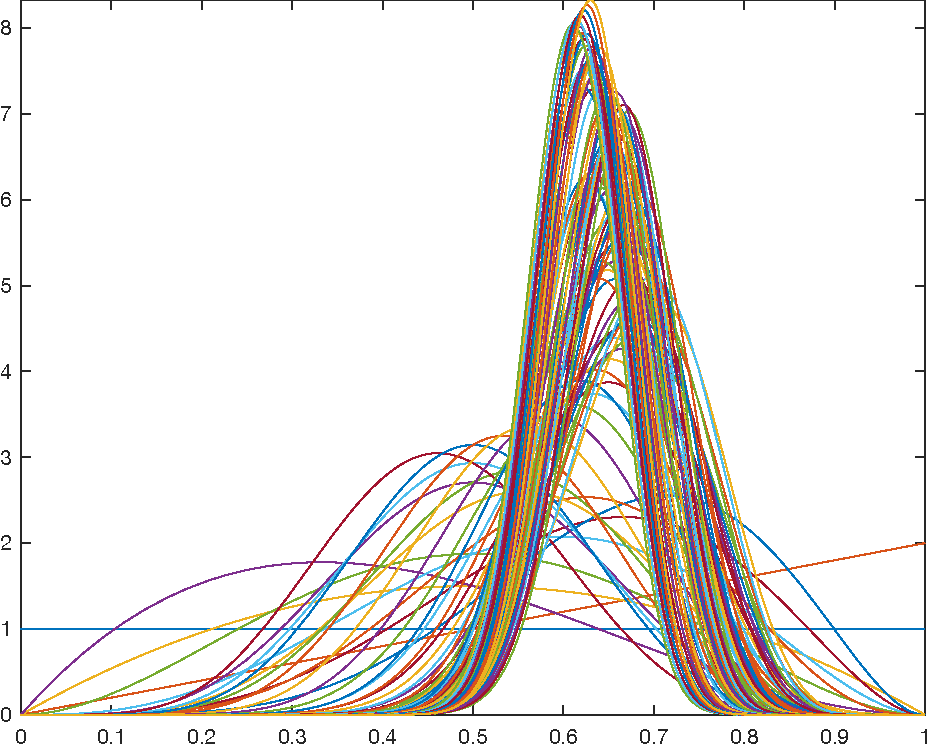
\includegraphics[width=0.75\textwidth]{bvm}
\end{figure}
\end{columns}

% rng(42);
% ntotal = 100;
% x = binornd(1,0.6,[ntotal,1]);
% sx = cumsum(x);
% syms t;
% fplot(1,[0,1]);
% hold on;
% for n = 1:ntotal
%     fn = t^sx(n)/(1-t)^(sx(n)-n);
%     fn0 = fn/int(fn,[0,1]);
%     fplot(fn0,[0,1]);
% end

% bar([0,1],[0.4,0.6],0.1);
% ylim([0,1]);

\end{frame}

%%%%%%%%%%%%%%%%%%%%%%%%%%%%%%%%%%%%%%%%%%%%%%%%%
\begin{frame}{Bernstein{\textendash}von Mises Theorem}
\Large
We have reason to believe $p(z_t|x_t)$ is better-approximated as Gaussian than $p(x_t|z_t)$.

\bigskip

\begin{columns}[T] % align columns
\column{.48\textwidth}

The number of observed dimensions is growing rapidly.
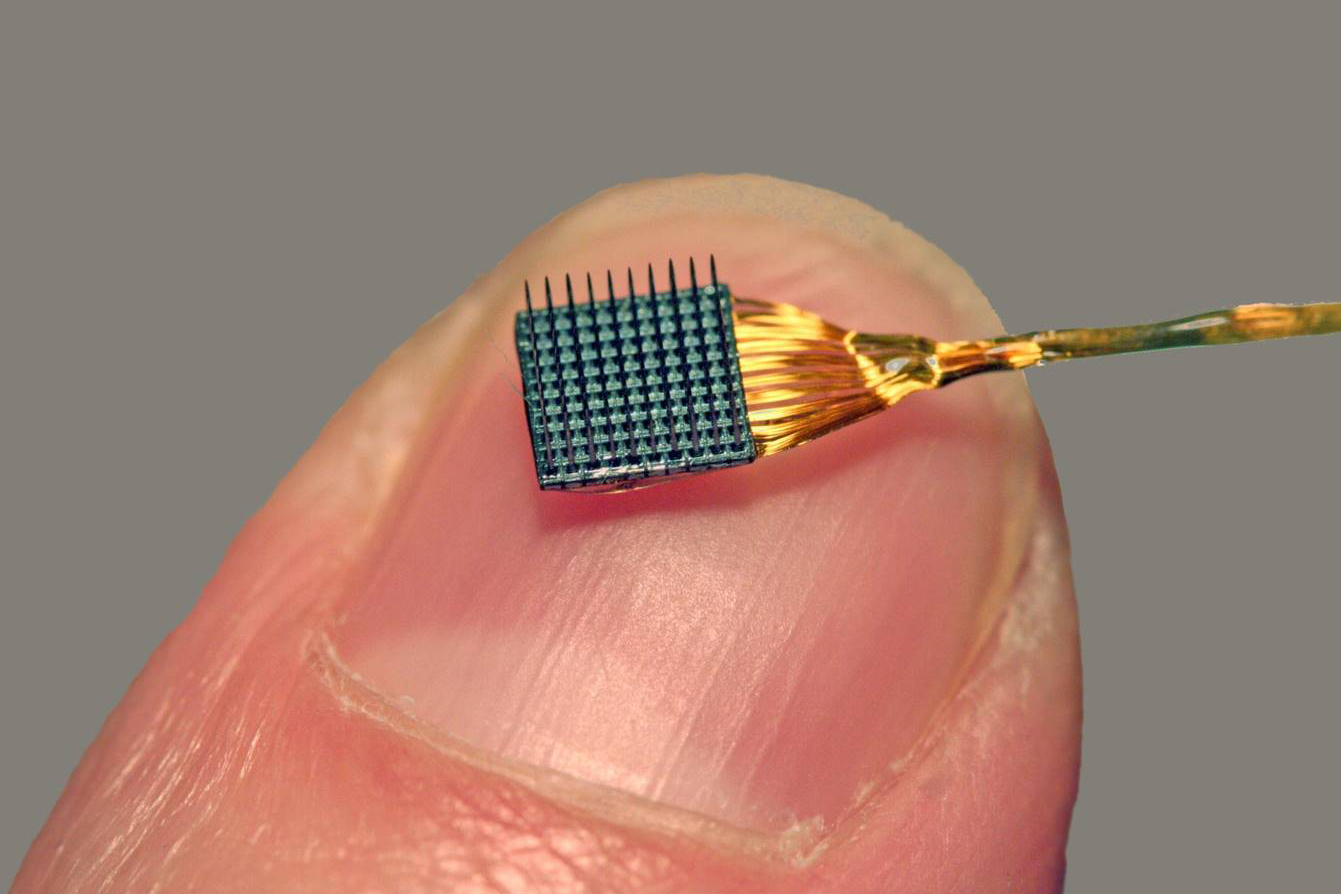
\includegraphics[width=0.8\textwidth]{braingate6}

\column{.48\textwidth}

The Bernstein--von Mises Theorem (Bayesian CLT) provides mild conditions under which $p(z_t|x_t)$ becomes Gaussian in the limit as $\dim(X_t)\rightarrow\infty$ \cite{vdV98}.  

\end{columns}

\footnotetext{image credit: BrainGate}

\end{frame}

% %%%%%%%%%%%%%%%%%%%%%%%%%%%%%%%%%%%%%%%%%%%%%%%%%
% \begin{frame}{Even for low-dimensional $X_t$\dots}
% \Large
% It's not hard to imagine models where $p(z_t|x_t)$ is better-approximated as Gaussian than $p(x_t|z_t)$.
% \begin{itemize}
%     \item if $X_t$ and $Z_t$ are uncorrelated (but dependent), then the Kalman/EKF/UKF filters are completely ineffective~\cite{Kus67}
%     \item models for which this is the case and for which $Z_t|X_t$ is bell-shaped are relatively easy to design
%     \item the DKF to effectively use, e.g., binary-valued $X_t$ data for filtering
% \end{itemize}
% \end{frame}

%%%%%%%%%%%%%%%%%%%%%%%%%%%%%%%%%%%%%%%%%%%%%%%%%
\begin{frame}{Theoretical Assurances}
\Large
\begin{columns}[T] % align columns
\column{.48\textwidth}

One potential concern might be that the renormalization step (dividing by a small quantity) could amplify approximation errors.  We can show that this is not a problem.
 
\column{.48\textwidth}

\raggedleft
\textbf{Result.}
\emph{Under mild assumptions, the total variation between our approximation for $p(z_t|x_{1:t})$ and the true distribution converges in probability to zero as $n\to\infty$.}

\end{columns}
\end{frame}

%%%%%%%%%%%%%%%%%%%%%%%%%%%%%%%%%%%%%%%%%%%%%%%%%
\begin{frame}{Model Validation: an Example}
\Large
\begin{columns}[T] % align columns
\column[t]{.48\textwidth}

Consider a Kalman \textcolor{navy}{state model} and a \textcolor{green}{measurement model} given by a mixture of linear Gaussians
 \[ 
 \textcolor{green}{p(x_t|z_t)} = \textstyle \textcolor{green}{\sum_{\ell=1}^L \pi_\ell \eta_n(x_t;H_\ell z_t,\Lambda_\ell)}. 
 \]
For parameters that make $X_t$ and $Z_t$ uncorrelated (but dependent), the Kalman/EKF/UKF filters are completely ineffective~\cite{Kus67}.
 
\column[t]{.48\textwidth}
\begin{figure}
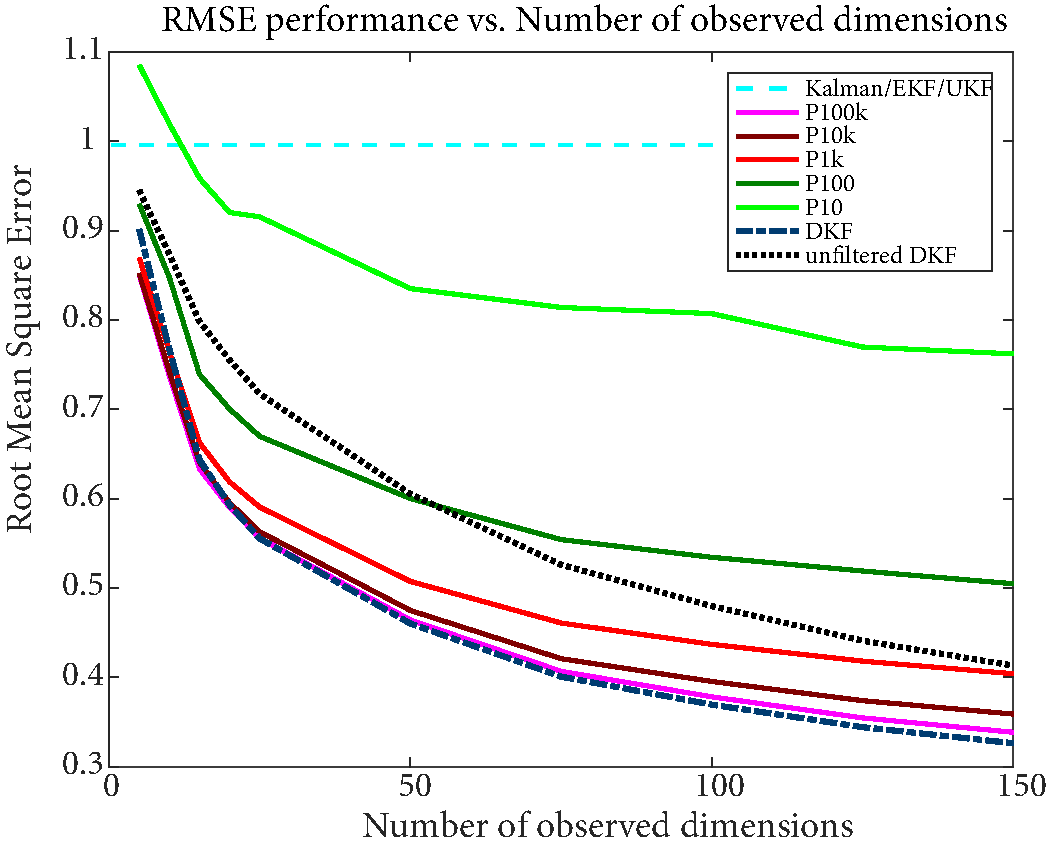
\includegraphics[width=\textwidth]{mdl62results}
\end{figure}

\end{columns}
\end{frame}

%%%%%%%%%%%%%%%%%%%%%%%%%%%%%%%%%%%%%%%%%%%%%%%%%
\begin{frame}{Learning $p(z_t|x_t)$}
\Large
Given a training set of $(x_i,z_i)$ pairs, we experimented with various supervised methods to learn the functions $f(\cdot)$ and $Q(\cdot)$.
\begin{itemize}
    \item \textbf{Nadaraya{\textendash}Watson kernel regression}: a kernel-density estimation approach~\cite{Nad64,Wat64}
    \item \textbf{Neural network}: parametric and thus relatively better-suited to larger training sets~\cite{Bis06}
    \item \textbf{Gaussian process regression}: method ultimately implemented at BrainGate \cite{Ras06}
\end{itemize}
\end{frame}

%%%%%%%%%%%%%%%%%%%%%%%%%%%%%%%%%%%%%%%%%%%%%%%%%
\setbeamertemplate{background}{%
    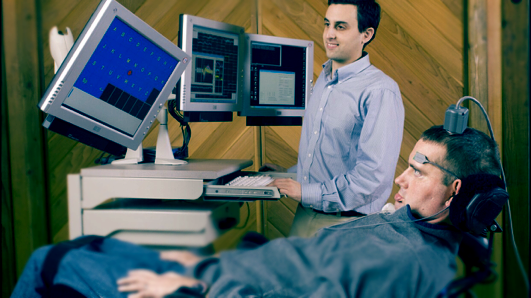
\includegraphics[width=\paperwidth,height=\paperheight,keepaspectratio]{bg_setup}}
\begin{frame}[b]{}

\begin{block}{}
\Large
\color{black} The DKF with GP mean function was used by 3 human volunteers to control a cursor with mental imagery alone~\cite{Bra18}.
\end{block}

\footnotetext{\color{red}image credit: BrainGate}

\end{frame}
\setbeamertemplate{background}{}

%%%%%%%%%%%%%%%%%%%%%%%%%%%%%%%%%%%%%%%%%%%%%%%%%
\begin{frame}{Cross-country Neural Decoding}
\Large
Nuyujukian et al. used the DKF-GP decoder to facilitate participant T9's use of a tablet computer for sending messages to another BrainGate participant based in California.
\end{frame}

%%%%%%%%%%%%%%%%%%%%%%%%%%%%%%%%%%%%%%%%%%%%%%%%%
\section{Overcoming Nonstationarities}
%%%%%%%%%%%%%%%%%%%%%%%%%%%%%%%%%%%%%%%%%%%%%%%%%

\begin{frame}{The Problem of Nonstationarities}
\Large
The relationship between neural signals and user intention can change over the course of mere hours or minutes~\cite{Per13,Per14}.

\[
\begin{tikzpicture}[commutative diagrams/every diagram]
\matrix[matrix of math nodes, name=m, commutative diagrams/every cell, ampersand replacement=\&, column sep=1.6cm] {
Z_1 \& Z_2 \& \cdots \& Z_{n-1}  \& Z_n \\
X_1 \& X_2 \& \& X_{n-1} \& X_n \\ };
  \path[commutative diagrams/.cd, every arrow, every label]
    (m-1-1) edge (m-1-2)
    		edge (m-2-1)
    (m-1-2) edge (m-1-3)
    		edge (m-2-2)
    (m-1-3) edge (m-1-4)
    (m-1-4) edge (m-1-5)
    		edge[commutative diagrams/rightsquigarrow] (m-2-4)
    (m-1-5) edge[commutative diagrams/rightsquigarrow] (m-2-5);
    \draw [decorate,thick,decoration={brace,mirror,amplitude=10pt}]
(m-2-1.south west) -- (m-2-2.south east) node [midway,below=10pt]
{used to learn $\textcolor{green}{p(z_t|x_t)}$};
 \draw [decorate,thick,decoration={brace,mirror,amplitude=10pt}]
(m-2-4.south west) -- (m-2-5.south east) node [midway,below=10pt]
{\dots but there was a change};
\end{tikzpicture}
\]
\end{frame}

%%%%%%%%%%%%%%%%%%%%%%%%%%%%%%%%%%%%%%%%%%%%%%%%%
\begin{frame}{Approach 1. Closed-loop decoder adaptation}
\Large
\begin{itemize}
    \item idea: continuously re-train the model with new data
    \item requires a nonstationary to be present for some time (during which filter performs poorly)
    \item can adapt to any arbitrary change in relationship
\end{itemize}

\footnotetext{\emph{cf.}\cite{Jarosiewicz2015, Bacher2015, Gilja2015,Orsborn2014, Shpigelman2008,Shanechi2014, Shanechi2016, Dangi2011}}
\end{frame}

%%%%%%%%%%%%%%%%%%%%%%%%%%%%%%%%%%%%%%%%%%%%%%%%%
\begin{frame}{Approach 2: Train a Robust Model}
\Large
Alternatively:
\bigskip

\begin{itemize}
    \item idea: train a model that is robust to certain types of nonstationarity
    \item automatically handles nonstationarities
    \item does not require online feedback or online retraining
    \item the amount change that can be overcome in this way is limited
\end{itemize}
\textcite{Sus12,Sus16} piloted this approach by learning a stateful RNN for primate neural decoding (using data augmentation).
\end{frame}

%%%%%%%%%%%%%%%%%%%%%%%%%%%%%%%%%%%%%%%%%%%%%%%%%
\begin{frame}{Kernel Selection for Robustness}
\Large
\vspace{-15pt}
\begin{columns}
\column[t]{0.48\textwidth}
\raggedright
\begin{enumerate}
\item Given a supervised training set of $(x_i,z_i)$ neural-intention pairs, we use a kernel regression estimator to obtain
\[
\Exp[Z_t|X_t=x_t] \propto \sum_{i=1}^n z_i k(x_t, x_i).
\]
\item The DKF then filters this estimate to obtain $\Exp[Z_t|X_{1:t}=x_{1:t}]$.
\end{enumerate}

\column[t]{0.48\textwidth}
\raggedleft
\begin{figure}
\raggedleft
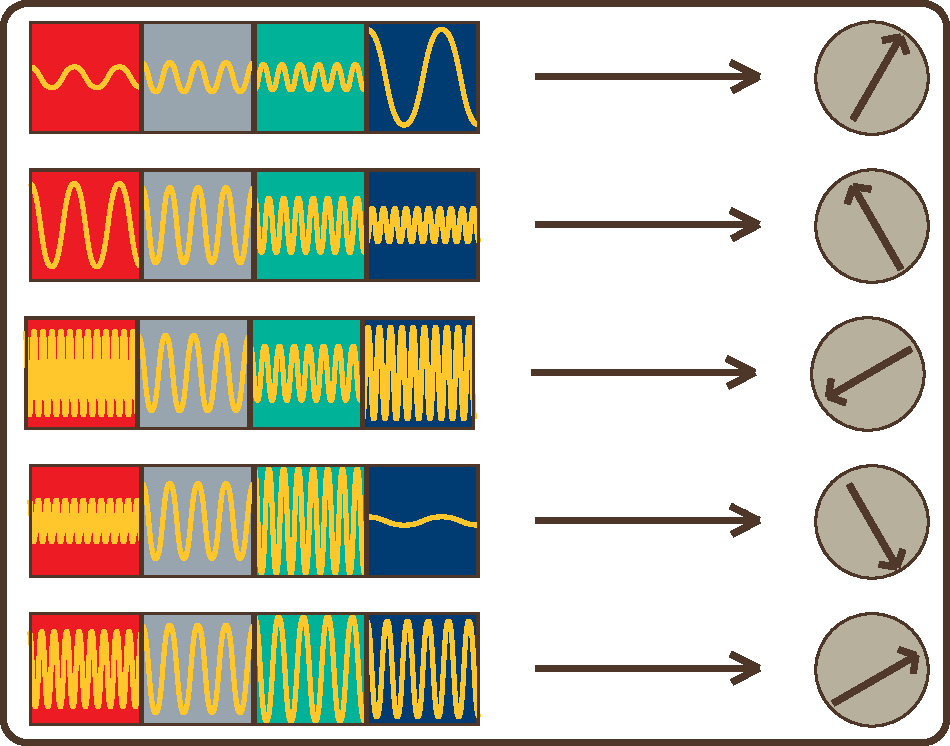
\includegraphics[width=0.5\textwidth]{training_bank}
\end{figure}

The above toy training bank of neural-intention pairs yields the following estimator for the test point $x_t$:

\begin{figure}
\raggedleft
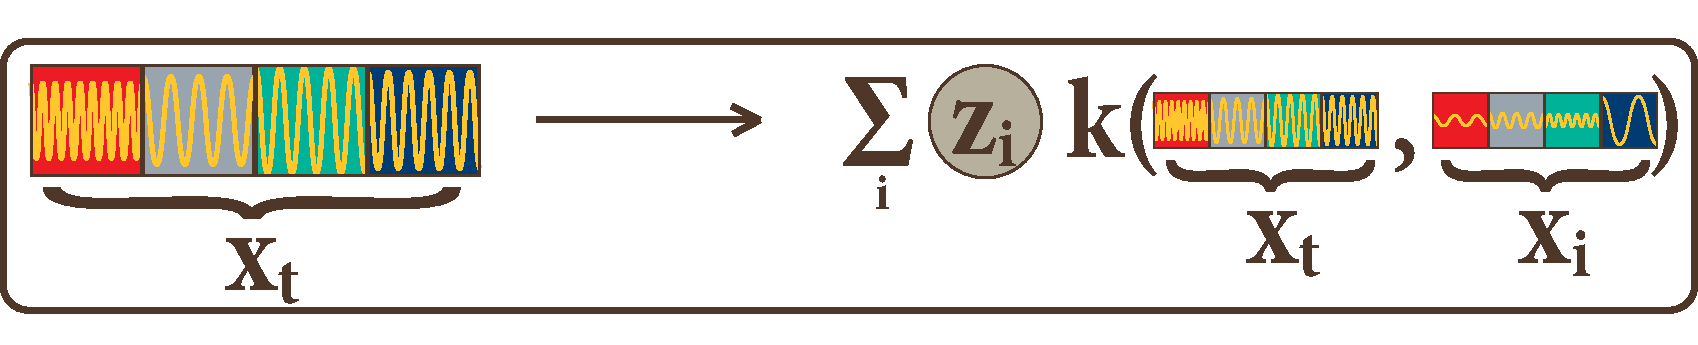
\includegraphics[width=0.9\textwidth]{kernel_regression}
\end{figure}

\end{columns}
\end{frame}

%%%%%%%%%%%%%%%%%%%%%%%%%%%%%%%%%%%%%%%%%%%%%%%%%
\begin{frame}{Kernel Selection}
\Large

idea: to protect against single-neuron dropout/wonkiness, find a kernel that ignores large differences along a single dimension

\begin{columns}[T] % align columns
\column[t]{.48\textwidth}
\centering
\textbf{Standard Gaussian} \\
product of 1-d Gaussians \\
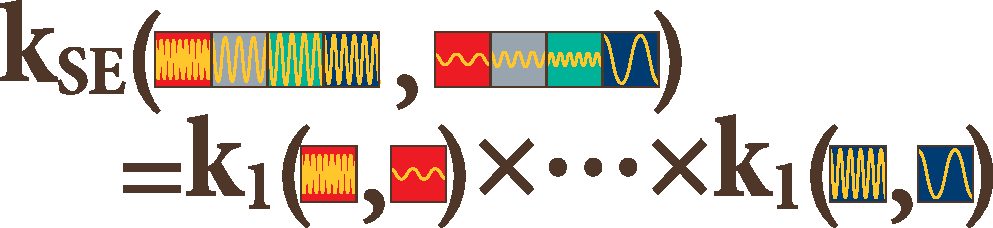
\includegraphics[height=1cm]{se2alt} \\
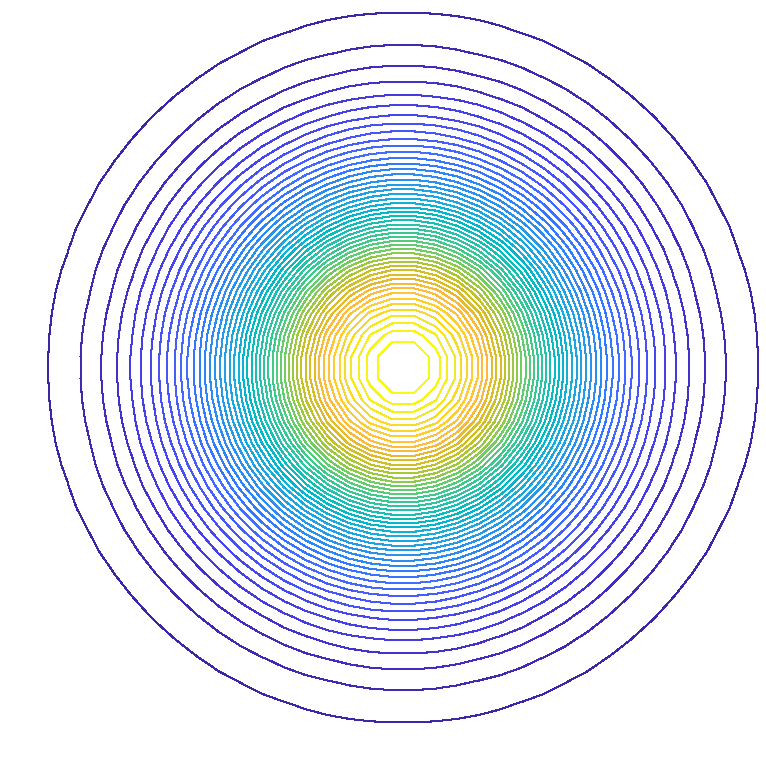
\includegraphics[height=0.6\textwidth]{se2d}

\column[t]{.48\textwidth}
\centering
\textbf{Multiple Kernel} \\
sum of 1-d Gaussians~\cite{Gon11} \\

\includegraphics[height=1cm]{mk2alt} \\
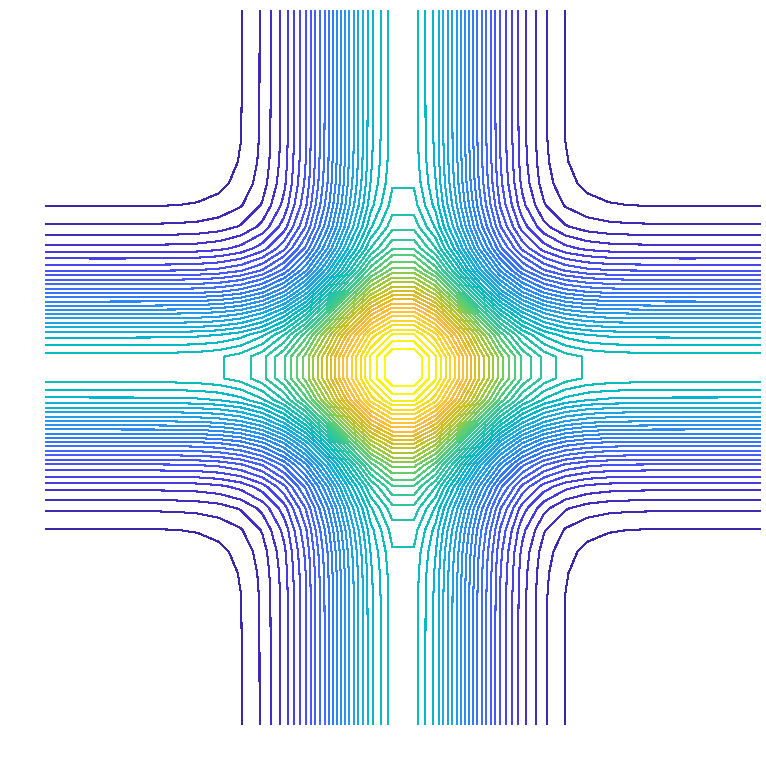
\includegraphics[height=0.6\textwidth]{mk2d}

\end{columns}
\end{frame}


%%%%%%%%%%%%%%%%%%%%%%%%%%%%%%%%%%%%%%%%%%%%%%%%%
\setbeamertemplate{background}{%
    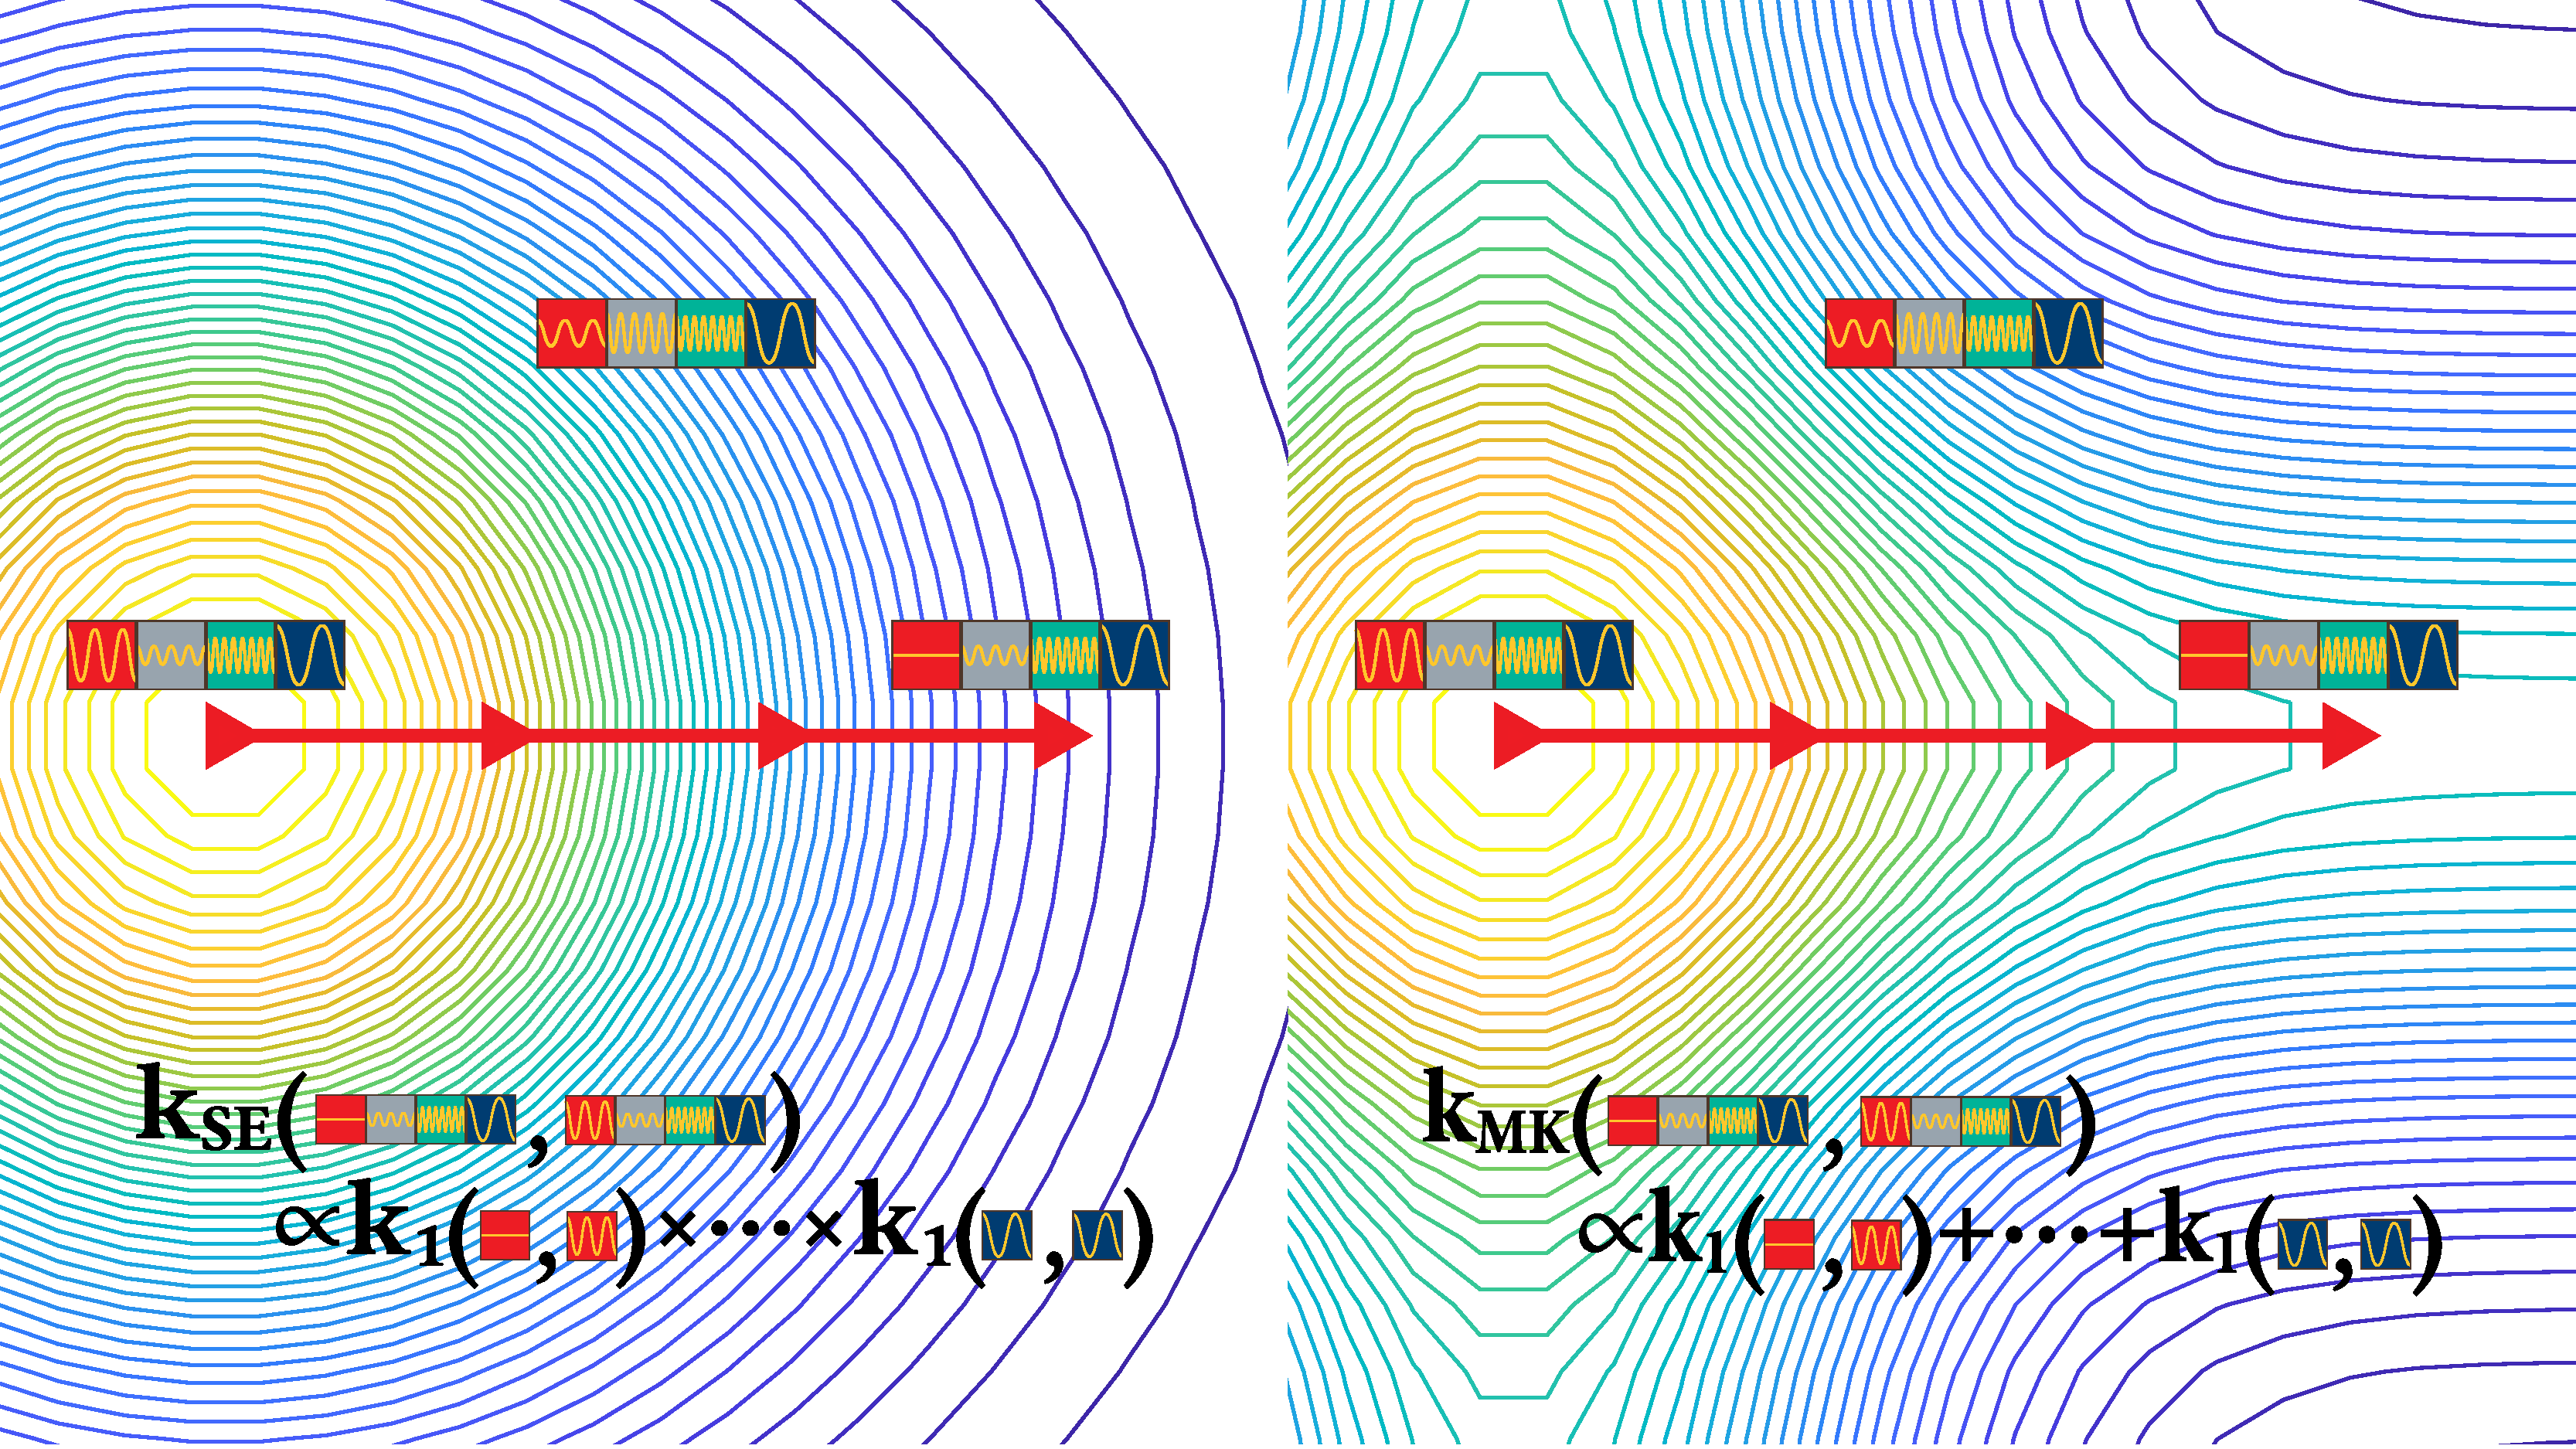
\includegraphics[width=\paperwidth,height=\paperheight,keepaspectratio]{se_vs_mk}}
\begin{frame}[b]{}
\Large
\begin{columns}[T] % align columns
\column{.49\paperwidth}
\textbf{Standard Gaussian}

\column{.49\paperwidth}
\textbf{Multiple Kernel}
\end{columns}

\end{frame}

\setbeamertemplate{background}{}

%%%%%%%%%%%%%%%%%%%%%%%%%%%%%%%%%%%%%%%%%%%%%%%%%
\begin{frame}{Results from Online Noise Injection Experiment with T10}
\Large
\begin{figure}
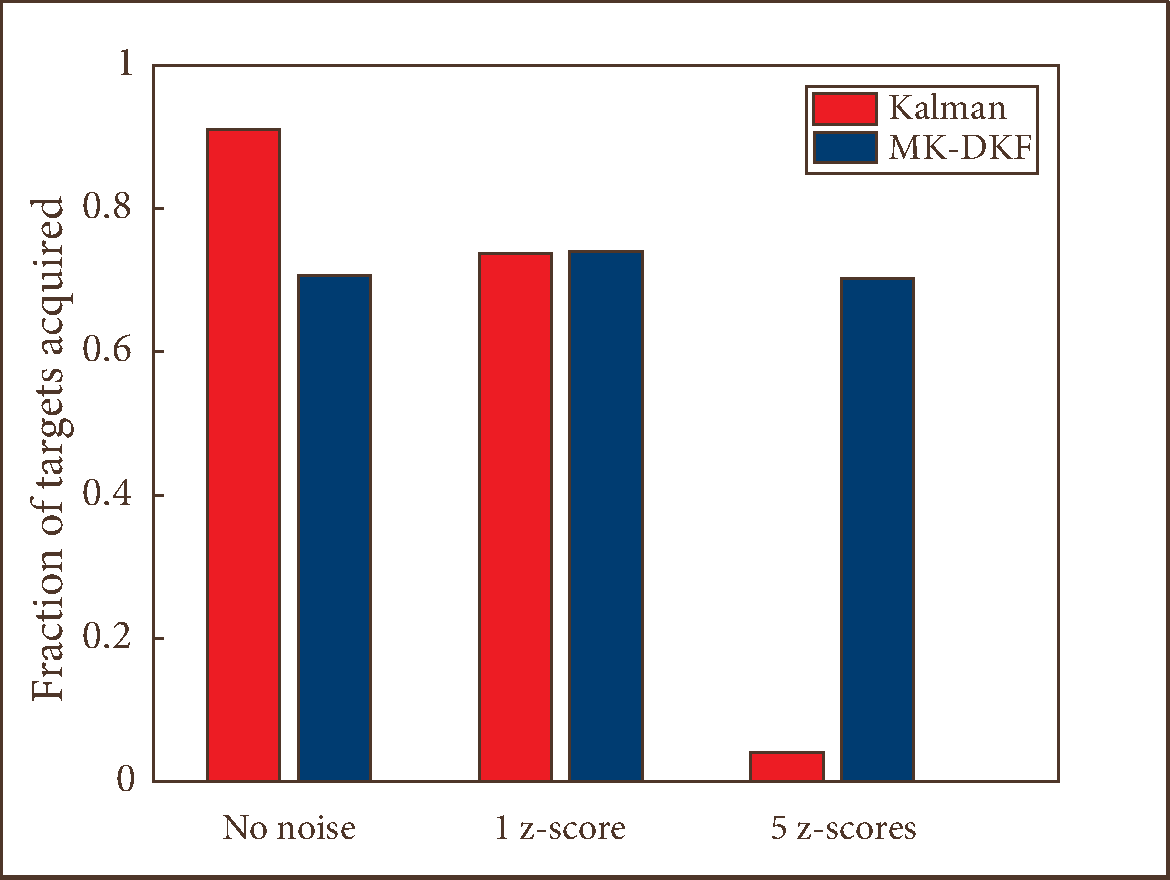
\includegraphics[width=0.7\textwidth]{kernel_results}
\end{figure}
\end{frame}

%%%%%%%%%%%%%%%%%%%%%%%%%%%%%%%%%%%%%%%%%%%%%%%%%
\begin{frame}{Litany of the Saints}
\vspace{-15pt}

\begin{columns}
\column[t]{0.25\paperwidth}
\begin{itemize}
    \item my parents
    \item Matthew Harrison
    \item Basilis Gidas
    \item Jerome Darbon
    \item Johnny Guzm\'an
    \item Elizabeth Crites
    \item Michael Snarski
    \item Ian Alevy
    \item Sameer Iyer
    \item Cat Munro
    \item Clark Bowman
    \item Dan Keating
    \item David Brandman
\end{itemize}
\column[t]{0.25\paperwidth}
\begin{itemize}
    \item James Beatty
    \item Chris Grimm
    \item Leigh Hochberg
    \item Kathleen Helbing
    \item Robert Zink
    \item Burgess Davis
    \item Hans Uli Walther
    \item Daniel Ocone
    \item Eduardo Sontag
    \item Victor Zavala
    \item John Wiegand \& family
    \item Chris O'Neil \& family
\end{itemize}
\column[t]{0.25\paperwidth}
\begin{itemize}
    \item Ivana Petrovic
    \item Nathan Meyers
    \item Guo-Jhen Wu
    \item Yuliya Mironovas
    \item Beth Travers
    \item Jean Radican
    \item Stephanie Han
    \item David Rosler
    \item John Simeral
    \item T9 \& family
    \item T10 \& family
    \item Jad Saab
    \item Daniel Milstein
\end{itemize}
\column[t]{0.25\paperwidth}
\begin{itemize}
    \item Ed Chien
    \item Isaac Solomon
    \item Nobuyuki Kaya % 賀谷 信幸
    \item Brittany Sorice
    \item Jessica Kelemen
    \item Brian Franco
    \item Beata Jarosiewicz
    \item Carlos Vargas-Irwin
    \item Arthur Gretton
    \item Tommy Hosman
    \item Benjamin Shanahan
\end{itemize}
And so many others!
\end{columns}
\end{frame}


%%%%%%%%%%%%%%%%%%%%%%%%%%%%%%%%%%%%%%%%%%%%%%%%%
\setbeamertemplate{background}{%
    
\includegraphics[width=\paperwidth,height=\paperheight,keepaspectratio]{brownlogo}}

\begin{frame}{}
\Huge \centering \minion This thesis is dedicated to BrainGate participant T9.
\end{frame}

%%%%%%%%%%%%%%%%%%%%%%%%%%%%%%%%%%%%%%%%%%%%%%%%%
\begin{frame}{}
\Huge \centering \minion Thanks for joining us today!
\end{frame}

\setbeamertemplate{background}{}

%%%%%%%%%%%%%%%%%%%%%%%%%%%%%%%%%%%%%%%%%%%%%%%%%
\begin{frame}{Bayesian Filtering Recursion}
\Large
\[
\underbrace{
\begin{tikzpicture}[commutative diagrams/every diagram]
\matrix[matrix of math nodes, name=m, commutative diagrams/every cell, ampersand replacement=\&, column sep=1.6cm] {
Z_1 \& \cdots \& Z_{t-1}  \& Z_t \\
X_1 \& \& X_{t-1} \& X_t \\ };
  \path[commutative diagrams/.cd, every arrow, every label]
    (m-1-1) edge (m-1-2)
    		edge (m-2-1)
    (m-1-2) edge (m-1-3)
    (m-1-3) edge node {$\textcolor{navy}{p(z_t|z_{t-1})}$} (m-1-4)
    		edge (m-2-3)
    (m-1-4) edge node {$\textcolor{green}{p(x_t|z_t)}$} (m-2-4);
    \draw[pattern=crosshatch, pattern color=red, draw = red, opacity=0.5] (m-1-1.north west) rectangle (m-2-3.south east) ;
    \draw[draw = red] (m-1-1.north west) rectangle (m-2-3.south east) node [pos=0.5,fill=skyblue] {\normalsize\textcolor{red}{$p(z_{t-1}|x_{1:t-1})$}};
\matrix[matrix of math nodes, name=m, commutative diagrams/every cell, ampersand replacement=\&, column sep=1.6cm] {
Z_1 \& \cdots \& Z_{t-1}  \& Z_t \\
X_1 \& \& X_{t-1} \& X_t \\ };
  \path[commutative diagrams/.cd, every arrow, every label]
    (m-1-1) edge (m-1-2)
    		edge (m-2-1)
    (m-1-2) edge (m-1-3)
    (m-1-3) edge node {$\textcolor{navy}{p(z_t|z_{t-1})}$} (m-1-4)
    		edge (m-2-3)
    (m-1-4) edge node {$\textcolor{green}{p(x_t|z_t)}$} (m-2-4);
    \end{tikzpicture}
}_{\textcolor{red}{p(z_t|x_{1:t})}}
\]
\end{frame}


%%%%%%%%%%%%%%%%%%%%%%%%%%%%%%%%%%%%%%%%%%%%%%%%%
\begin{frame}{Kalman Filter Derivation}

If the measurement and observation models are linear, Gaussian
\[
\textcolor{navy}{p(z_t|z_{t-1})}
= \textcolor{navy}{\eta_d(z_t;Az_{t-1},\Gamma)} 
\quad\text{ and } \quad
\textcolor{green}{p(x_t|z_t)}
= \textcolor{green}{\eta_n(x_t;Hz_t,\Lambda)}
\]
then (if $z_t$ stationary), the posterior $ \textcolor{red}{p(z_t|x_{1:t})}= \textcolor{red}{\eta_d(z_t; \nu_t, \Phi_t)}$ is also Gaussian and
we have:
\begin{align*}
{\textcolor{red}{p(z_t|x_{1:t})}} &\propto {\textcolor{green}{p(x_t|z_t)}} \int {\textcolor{navy}{p(z_t|z_{t-1})}}\; {\textcolor{red}{p(z_{t-1}|x_{1:t-1})}} \; dz_{t-1}\\
\textcolor{red}{\eta_d(z_t; \nu_t, \Phi_t)} &\propto {\textcolor{green}{\eta_n(x_t;Hz_t,\Lambda)}} \underbrace{\int \textcolor{navy}{\eta_d(z_t;Az_{t-1},\Gamma)}\; \textcolor{red}{\eta_d(z_{t-1}; \nu_{t-1}, \Phi_{t-1})}\; dz_{t-1}}_{p(z_t|x_{1:t-1})\propto \eta_d(z_t;A\nu_{t-1},A\Phi_{t-1}A^\intercal + \Gamma)} \\
&\propto \textcolor{red}{\eta_d\big(z_t; \Phi_t(H ^\intercal \Lambda^{-1}x_t+\hat\Phi_{t-1}^{-1}\hat\nu_{t-1}), \Phi_t \big)}
\end{align*}
where $\hat \nu_{t-1} = A\nu_{t-1}$, $\hat \Phi_{t-1} = A\Phi_{t-1}A^\intercal + \Gamma$, and 
\[
\Phi_t = (H^\intercal \Lambda^{-1}H + \hat\Phi_{t-1}^{-1})^{-1}
\]
\footnotetext{see \textcite{Kal60,Kal61} for the original papers}
\end{frame}

%%%%%%%%%%%%%%%%%%%%%%%%%%%%%%%%%%%%%%%%%%%%%%%%%
\begin{frame}{Kalman II}

By defining the Kalman gain as 
\[
K_t := \hat\Phi_{t-1}H^\intercal(H\hat\Phi_{t-1}H^\intercal + \Lambda)^{-1}
\]
it follows that
\[
\Phi_t 
= (I_d - K_tH)\hat\Phi_{t-1}
\]
and
\[
\nu_t = \hat\nu_{t-1} + K_t(x_t - H\hat\nu_{t-1}).
\]

\end{frame}

%%%%%%%%%%%%%%%%%%%%%%%%%%%%%%%%%%%%%%%%%%%%%%%%%
\begin{frame}{Kalman III}

Note that the Kalman model implies
\[
p(x_t|x_{1:t-1})= \eta_n(x_t;H\hat\nu_{t-1},H\hat\Phi_{t-1}H^\intercal+\Lambda).
\]
Let $\bar X_t, \bar Z_t$ be distributed as $X_t,Z_t$ conditioned on $X_{1:t-1}$, respectively.  Then
\begin{align*}
\var[\bar X_t] &= H\hat\Phi_{t-1}H^\intercal+\Lambda, \\
\operatorname{Cov}[\bar Z_t, \bar X_t] &= \hat\Phi_{t-1}H^\intercal,
\end{align*}
so that we can re-express the Kalman gain, posterior covariance, and posterior mean as:
\begin{align*}
K_t &= \operatorname{Cov}[\bar Z_t, \bar X_t] (\var[\bar X_t])^{-1} , \\
\Phi_t 
& = \var[\bar Z_t] - K_t \var[\bar X_t] K_t^\intercal, \\
\nu_t &= \mathbb{E}[\bar Z_t] + K_t(x_t - \mathbb{E}[\bar X_t]). 
\end{align*}
This will form the basis for the Gaussian assumed density filter (and UKF).
\end{frame}

%%%%%%%%%%%%%%%%%%%%%%%%%%%%%%%%%%%%%%%%%%%%%%%%%
\begin{frame}{Extended Kalman Filter}

If the measurement and observation models remain Gaussian, but are now allowed to be nonlinear:
\[
\textcolor{navy}{p(z_t|z_{t-1})}
= \textcolor{navy}{\eta_d(z_t;a(z_{t-1}),\Gamma)} 
\quad\text{ and } \quad
\textcolor{green}{p(x_t|z_t)}
= \textcolor{green}{\eta_n(x_t;h(z_t),\Lambda)}
\]
Then we can, at every time step, we can form a linear approximation at the prior mean and use that instead, i.e.:
\[
\textcolor{navy}{p(z_t|z_{t-1})}
\approx \textcolor{navy}{\eta_d(z_t;a(\nu_{t-1}) + \tilde A(z_t-\nu_{t-1}),\Gamma)} 
\text{ and }
\textcolor{green}{p(x_t|z_t)}
= \textcolor{green}{\eta_n(x_t;h(\hat \nu_{t-1})+\tilde H(z_t-\hat\nu_{t-1}),\Lambda)}
\]
where $\tilde A$ and $\tilde H$ are the Jacobians of $a,h$ evaluated at the respective prior means.
\footnotetext{see \textcite{Gel74} for details}
\end{frame}

%%%%%%%%%%%%%%%%%%%%%%%%%%%%%%%%%%%%%%%%%%%%%%%%%
\begin{frame}{Laplace Approximation}

This Taylor series expansion in the exponent replaces a pdf with a Gaussian density that matches curvature at the mode:
At step $t$,
\[
p(z_t | x_{1:t})  
\propto p(x_t | z_t) \int p(z_t|z_{t-1})\ p(z_{t-1} | x_{1:t-1})\ dz_{t-1} =: r(z_t)
\]
where $p(z_t| x_{1:t-1}) = \eta(z_t; \nu,\tau^2)$ so that
\[
g(z_t): = \log(r(z_t))
= -\frac{1}{2\tau^2}(z_t-\nu)^2 + \log(p(x_t | z_t))
\]
where $r(z_t) = e^{g(z_t)}$.  We find $z_t^* = \argmax_{z}g(z)$ and form the Laplace approximation
\[
r_1(z_t) \approx e^{g(z_t^*) + g'(z_t^*)(z-z_t^*) + g''(z_t^*)(z-z_t^*)^2/2} = \eta(z_t; z_t^*, -1/g''(z_t^*))
\]
where $g'(z_t^*)=0$ because $z_t^*$ is an extremal point and $g''(z_t^*)<0$ because $z_t^*$ is a maximum.
\footnotetext{see \textcite{But07} for details}
\end{frame}

%%%%%%%%%%%%%%%%%%%%%%%%%%%%%%%%%%%%%%%%%%%%%%%%%
\begin{frame}{Gaussian Assumed Density Filter}

Instead of solving for the posterior, we can find a Gaussian that most closely approximates it in the sense of KL-divergence:
\[
\nu_t, \Phi_t = \argmin_{a,b} \big\{D_{KL}\big(p(z_t|x_{1:t}) || \eta_d(z_t; a,b)\big)\big\}
\]
\begin{columns}
\column[t]{.38\textwidth}
This approach yields:
\begin{align*}
K &= P_{zx}P_{xx}^{-1}, \\
\Phi_t &= \hat\Phi_{t-1} - KP_{xx}K^\intercal , \\
\nu_t &= \hat\nu_{t-1} + K(x_t - \mu_x) .
\end{align*}
\column[t]{.58\textwidth}
where:
\begin{align*}
\mu_x &= \int h(z_t)\; \eta_d(z_t;\hat\nu_{t-1},\hat\Phi_{t-1})\; dz_t,\\
P_{xx} &= \int (h(z_t)-\mu_x) (h(z_t)-\mu_x)^\intercal \; \eta_d(z_t;\hat\nu_{t-1},\hat\Phi_{t-1})\; dz_t + \Lambda , \\
P_{zx} &= \int (z_t-\hat\nu_{t-1}) (h(z_t)-\mu_x)^\intercal \; \eta_d(z_t;\hat\nu_{t-1},\hat\Phi_{t-1})\; dz_t.
\end{align*}
for $Z_t \mid X_{1:t-1} \sim \N(\hat\nu_{t-1},\hat\Phi_{t-1})$.
\end{columns}

\footnotetext{see, e.g., \textcite{Kus67}}
\end{frame}

%%%%%%%%%%%%%%%%%%%%%%%%%%%%%%%%%%%%%%%%%%%%%%%%%
\begin{frame}{Gaussian Assumed Density Filter II}

In other words, we have:
\begin{align*}
K &= \cov[\hat Z_t, h(\hat Z_t)] (\var[h(\hat Z_t)] + \Lambda)^{-1}, \\
\Phi_t &= \hat\Phi_{t-1} - K(\var[h(\hat Z_t)] + \Lambda)K^\intercal , \\
\nu_t &= \hat\nu_{t-1} + K(x_t - \Exp[h(\hat Z_t)]) .
\end{align*}
where $\hat Z_t\sim \N(\hat\nu_{t-1},\hat\Phi_{t-1})$.  Nonlinear state updates are handled as follows:
\begin{align*}
\hat\nu_{t-1} &= \Exp[a(\bar Z_t)]) \\
\hat\Phi_{t-1} &= \var[a(\bar Z_t)]) \\
\end{align*}
where $\bar Z_t\sim \N(\nu_{t-1},\Phi_{t-1})$.

\end{frame}


%%%%%%%%%%%%%%%%%%%%%%%%%%%%%%%%%%%%%%%%%%%%%%%%%
\begin{frame}{Quadrature}

\begin{columns}
\column{0.38\textwidth}
\begin{center}
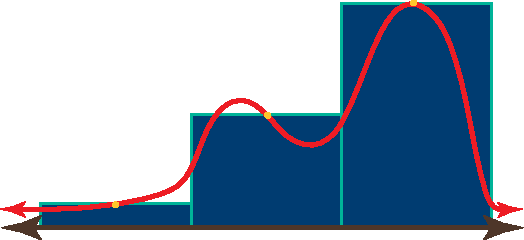
\includegraphics[width=0.7\textwidth]{q1}\\
\vspace{8pt}
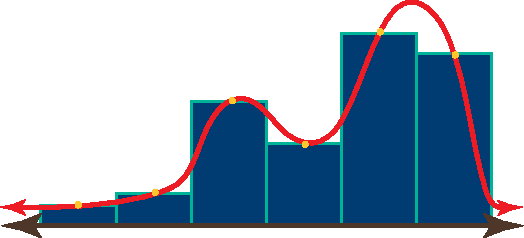
\includegraphics[width=0.7\textwidth]{q2}\\
\vspace{8pt}
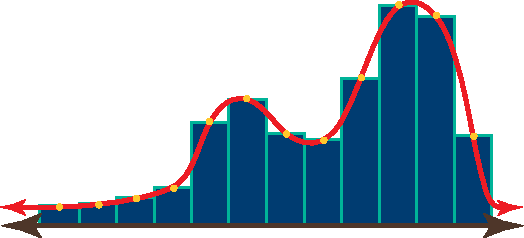
\includegraphics[width=0.7\textwidth]{q3}
\end{center}


\column{0.58\textwidth}
\begin{itemize}
\item quadrature converts integrals to sums by evaluating the integrand at a deterministic set of points (anchors)
\item for example, the midpoint quadrature rule estimates:
\[
\int_a^b f(x)\; dx \approx (b-a)\cdot f(\tfrac{a+b}{2})
\]
\item the Gaussian quadrature rule uses a clever choice of weights and points to make this approximation exact for all polynomials up to a certain degree~\cite{Gol73}
\item many quadrature rules have been used to calculate integrals for the Gaussian ADF
\end{itemize}

\end{columns}
\footnotetext{see \cite{Cha00,Ito00b,Ara07,Ara09}}

\end{frame}


%%%%%%%%%%%%%%%%%%%%%%%%%%%%%%%%%%%%%%%%%%%%%%%%%
\begin{frame}{Unscented Kalman Filter}

The UKF propagates $2d+1$ weighted points through $h$ to estimate the integrals in the Gaussian assumed density filter, in a method known as the unscented transform.  

\begin{columns}
\column{.48\textwidth}
We introduce parameters $\alpha>0,\beta\in\RR$ and consider the set of sigma vectors $\zeta_0,\dotsc,\zeta_{2d}\in\RR^{d}$ given by
\begin{align*}
\zeta_0 &= \hat\nu_{t-1}, \\
\zeta_i &= \hat\nu_{t-1} + \big(\sqrt{\alpha^2d\hat\Phi}\big)_i,\qquad i = 1,\dotsc, d \\
\zeta_i &= \hat\nu_{t-1} - \big(\sqrt{\alpha^2d\hat\Phi}\big)_i,\qquad i = d+1,\dotsc, 2d
\end{align*}
where $\big(\sqrt{\alpha^2d\hat\Phi}\big)_i$ denotes the $i$th row of the matrix square root.  

\column{.48\textwidth}
We set weights $w_0^{(m)}=1-1/\alpha^2$, $w_0^{(c)}=2-1/\alpha^2-\alpha^2+\beta$, and $w_0^{(m)}=w_0^{(c)}=1/(2\alpha^2d)$.  Then:
\begin{align*}
\mu_x &= \sum_{i=0}^{2d} w_i^{(m)}h(\zeta_i), \\
P_{xx} &= \sum_{i=0}^{2d} w_i^{(c)}(h(\zeta_i)-\bar x)(h(\zeta_i)-\bar x)^\intercal, \\
P_{zx} &= \sum_{i=0}^{2d} w_i^{(c)}(\zeta_i-\hat\nu_{t-1})(h(\zeta_i)-\bar x)^\intercal.
\end{align*}
\end{columns}

\footnotetext{see \textcite{Jul97} for original paper; \textcite{Wan00} for details}
\end{frame}

%%%%%%%%%%%%%%%%%%%%%%%%%%%%%%%%%%%%%%%%%%%%%%%%%
\begin{frame}{Sequential Importance Sampling}
Representing $\textcolor{red}{p(z_{t-1}|x_{1:t-1})} \approx \textcolor{red}{\sum_{\ell=1}^L w_{t-1}^{(\ell)} \delta_{z_{t-1}^{(\ell)}}(z_{t-1})}$ as the weighted sum of particles, we have:
\begin{align*}
{\textcolor{red}{p(z_t|x_{1:t})}} 
&\propto {\textcolor{green}{p(x_t|z_t)}} \int {\textcolor{navy}{p(z_t|z_{t-1})}}\; \textcolor{red}{\sum_{\ell=1}^L w_{t-1}^{(\ell)} \delta_{z_{t-1}^{(\ell)}}(z_{t-1})} \; dz_{t-1}\\
&\propto {\textcolor{green}{p(x_t|z_t)}} \textcolor{red}{\sum_{\ell=1}^L w_{t-1}^{(\ell)} \delta_{ z_t^{(\ell)}}(z_t)}, \quad \text{ where } z_t^{(\ell)}\sim Z_t| \{Z_{t-1}=z_{t-1}^{(\ell)}\} \\
&\propto  \textcolor{red}{\sum_{\ell=1}^L w_{t}^{(\ell)} \delta_{\hat z_{t-1}^{(\ell)}}(z_t)}, \quad \text{ where } w_t^{(\ell)} \propto w_{t-1}^{(\ell)} \cdot  p(X_t=x_t|Z_t=z_t^{(\ell)}).
\end{align*}

\footnotetext{see \textcite{del96,Dou00} for details}
\end{frame}

%%%%%%%%%%%%%%%%%%%%%%%%%%%%%%%%%%%%%%%%%%%%%%%%%
\begin{frame}{Sequential Importance Sampling II}
\begin{columns}
\column[t]{0.58\textwidth}
\begin{figure}
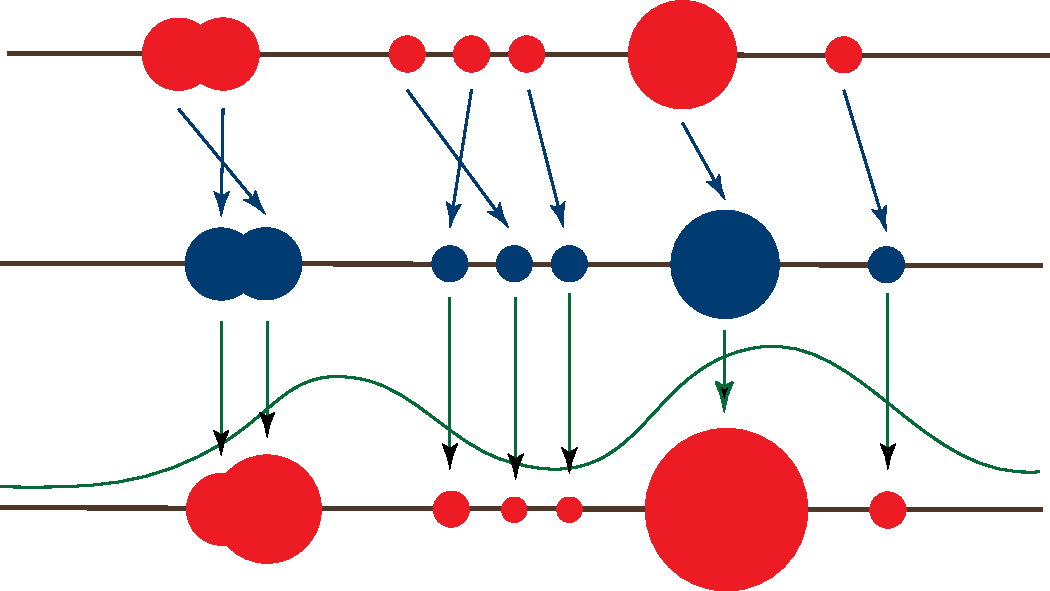
\includegraphics[width=\textwidth]{sis}
\end{figure}
\column[t]{0.38\textwidth}
\phantom{foo} \\ 
\vspace{14pt}
prior at time $t-1$\\
\vspace{33pt}
sample from \textcolor{navy}{state model}\\
\vspace{33pt}
re-weight according to \textcolor{green}{measurement model}\\
\end{columns}
\end{frame}


%%%%%%%%%%%%%%%%%%%%%%%%%%%%%%%%%%%%%%%%%%%%%%%%%
\begin{frame}{Sequential Importance Resampling}
In SIS, most of the weight can be placed a very few number of particles, leading to a problem called weight degeneracy.  A resampling step was introduced to fix that problem.
\begin{align*}
{\textcolor{red}{p(z_t|x_{1:t})}} 
&\propto {\textcolor{green}{p(x_t|z_t)}} \int {\textcolor{navy}{p(z_t|z_{t-1})}}\; \textcolor{red}{\sum_{\ell=1}^L w_{t-1}^{(\ell)} \delta_{z_{t-1}^{(\ell)}}(z_{t-1})} \; dz_{t-1}\\
&\propto {\textcolor{green}{p(x_t|z_t)}} \int {\textcolor{navy}{p(z_t|z_{t-1})}}\; \textcolor{red}{\sum_{\ell=1}^L \delta_{\tilde z_{t-1}^{(\ell)}}(z_{t-1})} \; dz_{t-1}, \\
\intertext{ where now $\tilde z_{t-1}^{(\ell)}$  are drawn, with replacement, from the $z_{t-1}^{(\ell)}$ with relative odds $w_{t-1}^{(\ell)}$, }
&\propto {\textcolor{green}{p(x_t|z_t)}} \textcolor{red}{\sum_{\ell=1}^L \delta_{ z_t^{(\ell)}}(z_t)}, \quad \text{ where } z_t^{(\ell)}\sim Z_t| \{Z_{t-1}=\tilde z_{t-1}^{(\ell)}\} \\
&\propto  \textcolor{red}{\sum_{\ell=1}^L w_{t}^{(\ell)} \delta_{\hat z_{t-1}^{(\ell)}}(z_t)}, \quad \text{ where } w_t^{(\ell)} \propto p(X_t=x_t|Z_t=z_t^{(\ell)}).
\end{align*}

\footnotetext{see \textcite{Gor93}}
\end{frame}

%%%%%%%%%%%%%%%%%%%%%%%%%%%%%%%%%%%%%%%%%%%%%%%%%
\begin{frame}{Sequential Importance Resampling II}
\begin{columns}
\column[t]{0.58\textwidth}
\begin{figure}
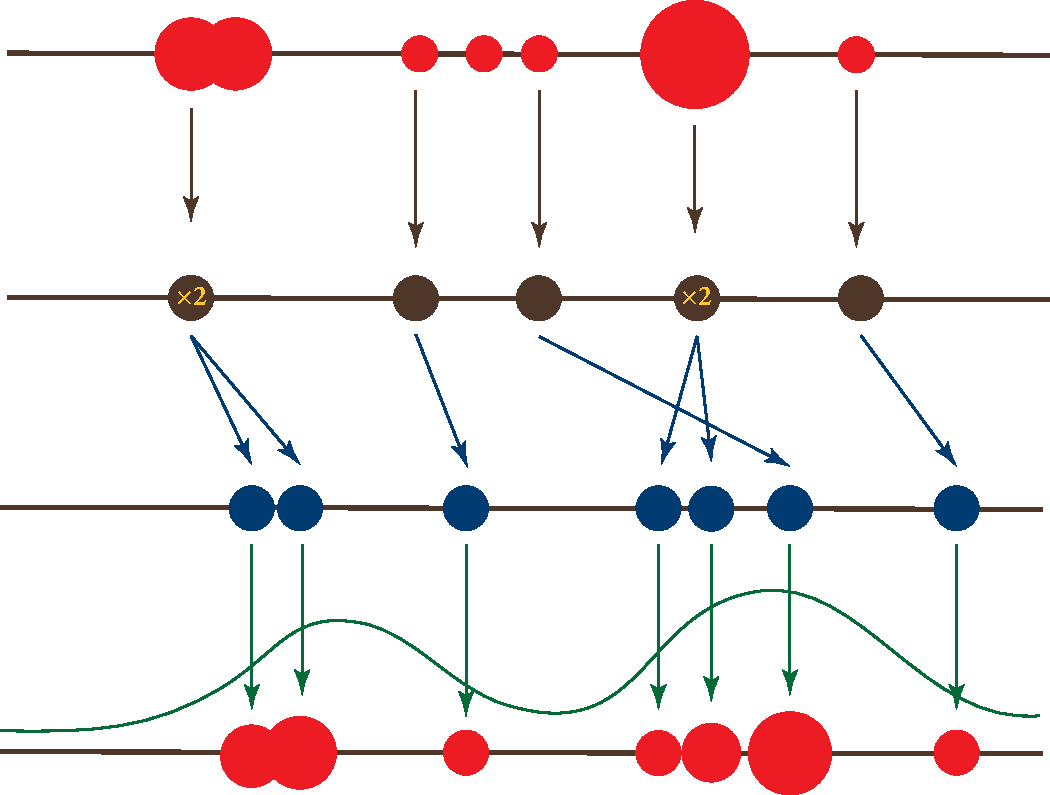
\includegraphics[width=\textwidth]{sir}
\end{figure}
\column[t]{0.38\textwidth}
\phantom{foo} \\ 
\vspace{15pt}
prior at time $t-1$\\
\vspace{38pt}
resample, reset weights\\
\vspace{34pt}
sample from \textcolor{navy}{state model} \\
\vspace{38pt}
re-weight according to \textcolor{green}{measurement model}
\end{columns}
\end{frame}


%%%%%%%%%%%%%%%%%%%%%%%%%%%%%%%%%%%%%%%%%%%%%%%%%
\begin{frame}{Variational Inference: an Illustrative Example}

\begin{columns}
\column[t]{0.58\textwidth}
0. Given a generative model $p(\beta,\theta,z)$ that's intractable to integrate:
\begin{center}
\resizebox{0.25\textwidth}{!}{
\begin{minipage}{.45\textwidth}
\centering
\begin{tikzpicture}

  % Nodes
  \node[latent,fill=none, draw=brown]                      (beta)     {$\beta_k$} ;
  \node[latent, left=1.0cm of beta, fill=none, draw=brown]  (eta)      {$\eta$} ;
  \node[obs, below=1.2cm of beta, fill opacity=0.35, draw=brown]    (w)        {$w_{d,n}$} ;
  \node[obs, below=1.2cm of beta, fill=none, draw=brown]    (w)        {$w_{d,n}$} ;
  \node[latent, left=1.0cm of w, fill=none, draw=brown]     (z)        {$z_{d,n}$} ;
  \node[latent, left=1.0cm of z, fill=none, draw=brown]     (theta)    {$\theta_d$} ;
  \node[latent, left=1.0cm of theta, fill=none, draw=brown] (alpha)    {$\alpha$};

  % Edges
  \edge{beta}{w};
  \edge{z}{w};
  \edge{theta}{z};
  \edge{alpha}{theta};
  \edge{eta}{beta};

  % Plates
  \plate[inner sep=0.2cm, yshift=0.1cm,
    label={[xshift=-15pt,yshift=13pt]south east:$N$}] {plate1} {
    (w)(z)
  } {};
  \plate[inner sep=0.45cm,
    label={[xshift=-15pt,yshift=13pt]south east:$D$}] {plate2} {
    (w)(z)(theta)
  } {};
  \plate[inner sep=0.2cm,
    label={[xshift=-15pt,yshift=13pt]south east:$K$}] {plate3} {
    (beta)
  } {};
\end{tikzpicture}
\end{minipage}
}
\end{center}

1. We can specify a (variational) model $q(\beta,\theta,z)$ that's easier to integrate (more independence):
\begin{center}
\resizebox{0.25\textwidth}{!}{
\begin{minipage}{.4\textwidth}
\centering
\begin{tikzpicture}

  % Nodes
  \node[latent,fill=none, draw=brown]                      (beta)     {$\beta_k$} ;
  \node[latent, left=1.0cm of beta,fill=none, draw=brown]  (lambda)   {$\lambda_k$} ;
  \node[latent, below=.8cm of beta,fill=none, draw=brown] (theta)    {$\theta_d$} ;
  \node[latent, left=1.0cm of theta,fill=none, draw=brown] (gamma)    {$\gamma_d$} ;
  \node[latent, below=0.3cm of theta,fill=none, draw=brown](z)        {$z_{d,n}$} ;
  \node[latent, left=1.0cm of z,fill=none, draw=brown]     (phi)      {$\varphi_{d,n}$} ;

  % Edges
  \edge{lambda}{beta};
  \edge{gamma}{theta};
  \edge{phi}{z};

  % Plates
  \plate[inner sep=0.15cm,
    label={[xshift=-15pt,yshift=13pt]south east:$N$}] {plate1} {
    (phi)(z)
  } {};
  \plate[inner sep=0.32cm, yshift=-7pt,
    label={[xshift=-15pt,yshift=13pt]south east:$D$}] {plate2} {
    (z)(phi)(theta)(gamma)
  } {};
  \plate[inner sep=0.15cm,
    label={[xshift=-15pt, yshift=13pt]south east:$K$}] {plate3} {
    (lambda)(beta)
  } {};
\end{tikzpicture}
\end{minipage}
}
\end{center}

\column[t]{0.48\textwidth}
2. We perform inference by tweaking the variational parameters to minimize KL divergence between the variational and true models:
\[
\hat\lambda,\hat\gamma,\hat\varphi = \argmin_{\lambda,\gamma,\varphi} \left\{ D \left(q(\beta,\theta,z) \|\; p(\beta,\theta,z) \right) \right\}
\]

3. Now, inference has become an optimization problem instead of an integration problem.

\end{columns}
\end{frame}

%%%%%%%%%%%%%%%%%%%%%%%%%%%%%%%%%%%%%%%%%%%%%%%%%
\begin{frame}{The Discriminative Kalman Filter}
\Large

\begin{columns}[T] % align columns
\column{.38\textwidth}

Under a stationary Kalman state model
\begin{align*}
{\textcolor{navy}{p(z_0)}} &= {\textcolor{navy}{\eta_d(z_t;\vec 0,S)}} \\
{\textcolor{navy}{p(z_t|z_{t-1})}} &= {\textcolor{navy}{\eta_d(z_t;Az_{t-1},\Gamma)}}
\end{align*}
and a discriminative observation model
\[
{\textcolor{green}{p(z_t|x_t)}}
\approx {\textcolor{green}{\eta_d(z_t;f(x_t),Q(x_t))}}
\]
the posterior will also be Gaussian.

\column{.58\textwidth}
At every time step $t$, we have
\begin{align*}
{\textcolor{red}{p(z_t|x_{1:t})}} 
&\approx {\textcolor{red}{\eta_d(z_t;\mu_t(x_{1:t}),\Sigma_t(x_{1:t}))}} \\
&\approx {\textcolor{red}{\eta_d(z_t;\mu_t,\Sigma_t)}}
\end{align*}
related sequentially via the closed-form updates
\begin{align*}  
M_t &= A\Sigma_{t-1}A^\tr+\Gamma , \\
\Sigma_t & = (Q(x_t)^{-1}+M_t^{-1}-S^{-1})^{-1} ,  \\
\mu_t & = \Sigma_t(Q(x_t)^{-1}f(x_t) + M_t^{-1}A\mu_{t-1})
\end{align*} 
if $(Q(x_t)^{-1}-S^{-1})^{-1}$ is pos.-definite.
\end{columns}
\end{frame}


%%%%%%%%%%%%%%%%%%%%%%%%%%%%%%%%%%%%%%%%%%%%%%%%%
\begin{frame}{Nonprobabilistic Filtering: the Long Short-Term Memory (LSTM) Recursive Neural Network}

\begin{center}
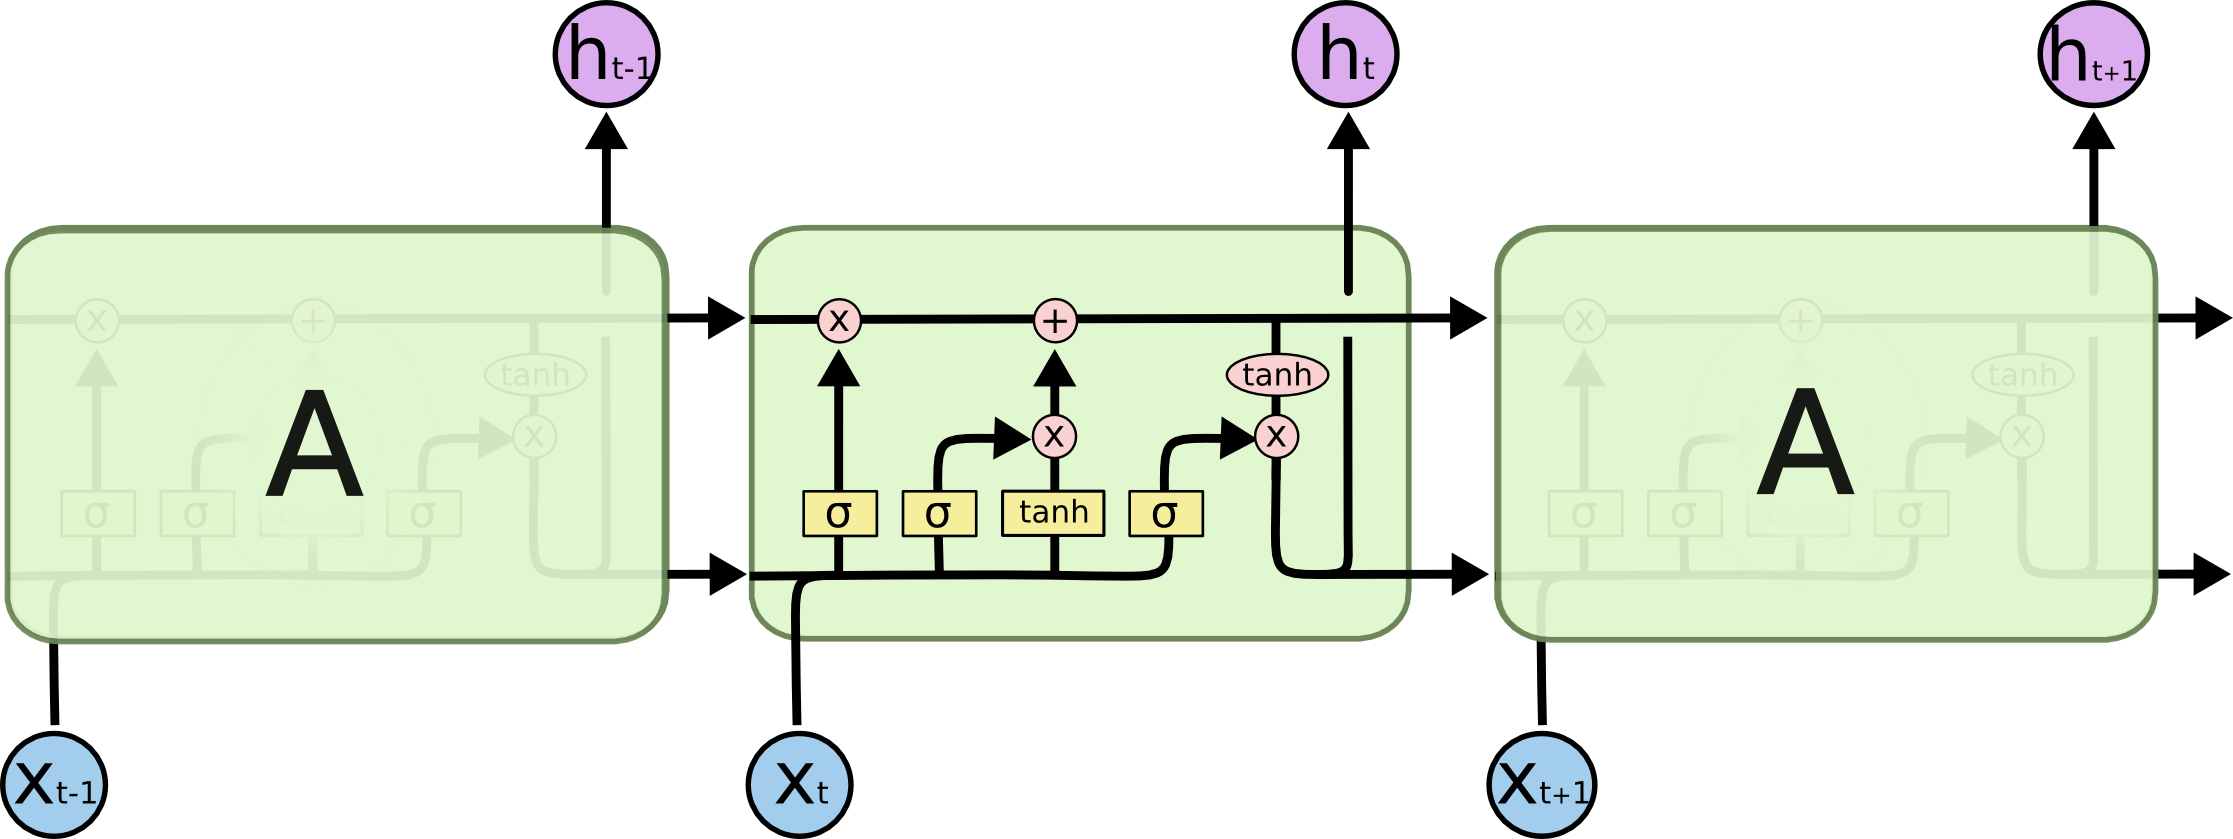
\includegraphics[width=0.6\textwidth]{lstm_chain}
\end{center}

\vspace{-20pt}

\begin{columns}
\column[t]{0.48\textwidth}
\begin{itemize}
    \item designed these to overcome error backflow problems~\cite{Hoc97}
    \item dropout~\cite{Sri14} should only applied to feedforward connections, not recurrent connections~\cite{Pha14, Zar14}
\end{itemize}

\column[t]{0.48\textwidth}
\begin{itemize}
    \item Batch-normalization to prevent covariate shift~\cite{Iof15}
    \item Xavier-type parameter initialization~\cite{Glo10}
    \item Adadelta~\cite{Zei12} was designed to improve Adagrad~\cite{Duc11} by allowing learning rate to sometimes increase
\end{itemize}

\end{columns}

\footnotetext{image credit: \textcite{Ola15}}
\end{frame}

%%%%%%%%%%%%%%%%%%%%%%%%%%%%%%%%%%%%%%%%%%%%%%%%%
\begin{frame}{LSTM implementation in TensorFlow: highlights}
\begin{figure}
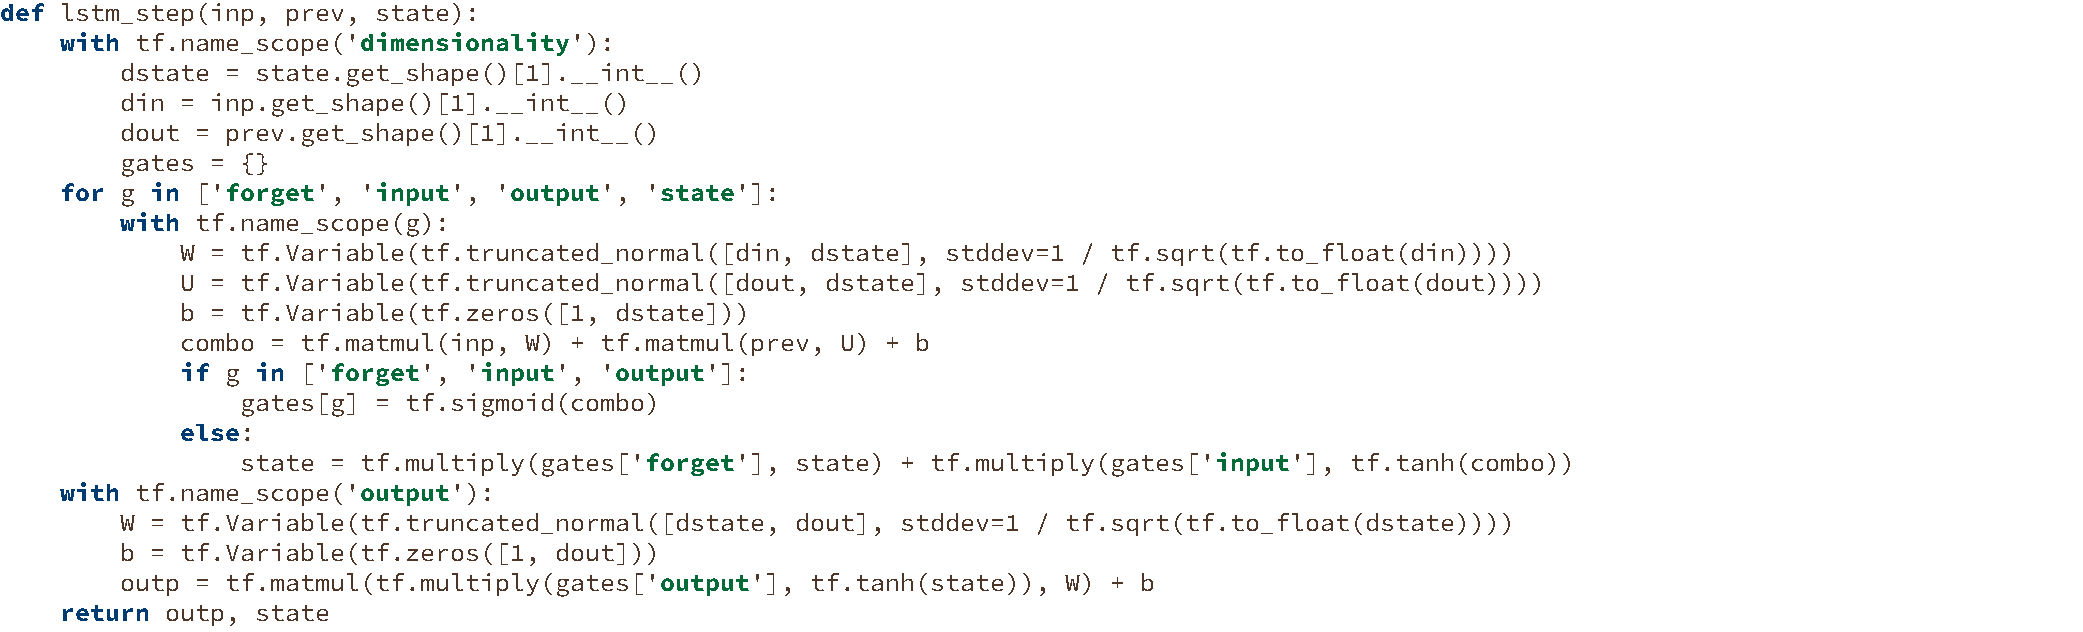
\includegraphics[width=\textwidth]{tf_lstm_cell}
\end{figure}
\begin{figure}
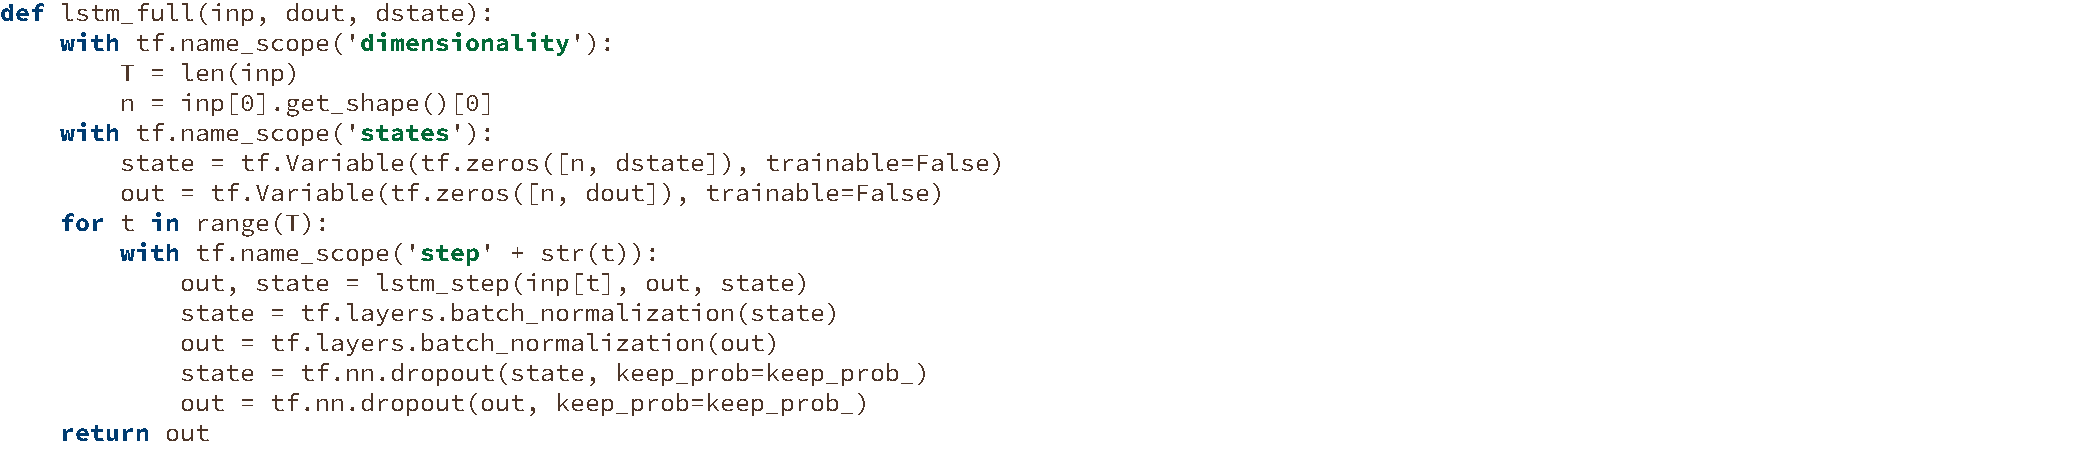
\includegraphics[width=\textwidth]{tf_lstm_full}
\end{figure}
\end{frame}

%%%%%%%%%%%%%%%%%%%%%%%%%%%%%%%%%%%%%%%%%%%%%%%%%
\begin{frame}{Nadaraya{\textendash}Watson Kernel Regression}
\begin{columns}
\column[t]{0.38\textwidth}
Given a dataset $\{(x_i,z_i)\}_{i=1}^n$, we can use Kernel Density Estimation (KDE) to model the joint density:
\[
p(z,x) \approx \frac{1}{n} \sum_{i=1}^n \kappa_Z(z,z_i)\kappa_X(x,x_i).
\]
The conditional distribution is then
\begin{align*}
p(z|x) 
&= \frac{p(z,x)}{p(x)}  \\
&\approx \frac{\sum_{i=1}^m \kappa_Z(z,Z_i)\kappa_X(x,X_i)}{ \sum_{i=1}^m \kappa_X(x,X_i)}.
\end{align*}
\column[t]{0.58\textwidth}
It follows that the conditional mean is
\begin{align*}
 \mathbb{E}[Z|X=x] 
 &= \int z p(z|x) dz  \\
 &\approx  \frac{\sum_{i=1}^m \big(\int z \kappa_Z(z,Z_i) dz\big) \kappa_X(x,X_i)}{ \sum_{i=1}^m \kappa_X(x,X_i)}  \\
 &\approx \frac{\sum_{i=1}^m Z_i \kappa_X(x,X_i)}{ \sum_{i=1}^m \kappa_X(x,X_i)}\end{align*}
for a symmetric kernel~\cite{Nad64, Wat64}.  If the kernel is also stationary
\[
\mathbb{E}[Z^\intercal Z|X=x]\approx  \Sigma_Z + \frac{\sum_{i=1}^m Z_i^\intercal Z_i \kappa_X(x,X_i)}{ \sum_{i=1}^m \kappa_X(x,X_i)}
\]
from which we estimate the conditional variance.
 \end{columns}
\end{frame}

%%%%%%%%%%%%%%%%%%%%%%%%%%%%%%%%%%%%%%%%%%%%%%%%%
\begin{frame}{Gaussian Process Model}
\Large

\begin{columns}[T] % align columns
\column{.38\textwidth}
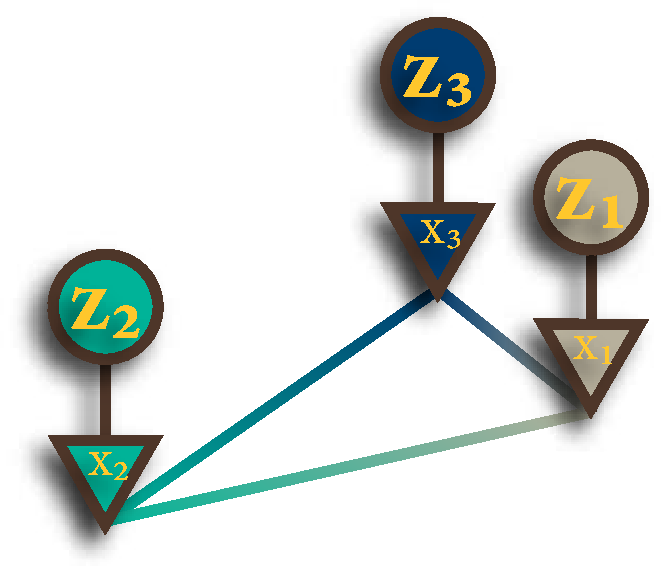
\includegraphics[width=\textwidth]{gp_model}

\column{.58\textwidth}
We specify a covariance structure:
\[
\begin{bmatrix} z_1 \\ z_2 \\ z_3 \end{bmatrix} 
\sim \N\left(\begin{bmatrix} 0 \\ 0 \\ 0 \end{bmatrix}, \begin{bmatrix} k_{11} & k_{12} & k_{13} \\ k_{21} & k_{22} & k_{23} \\ k_{31} & k_{32} & k_{33} \end{bmatrix} + \sigma^2 I \right)
\]
where
\[
k_{ij} = k_\theta(x_i,x_j)
\]
\end{columns}

\vspace{10pt}
\emph{so that closer $x$-values correspond to more correlated $z$-values.}

\end{frame}

%%%%%%%%%%%%%%%%%%%%%%%%%%%%%%%%%%%%%%%%%%%%%%%%%
\begin{frame}{Gaussian Process Inference}
\Large

\begin{columns}[T] % align columns
\column{.38\textwidth}
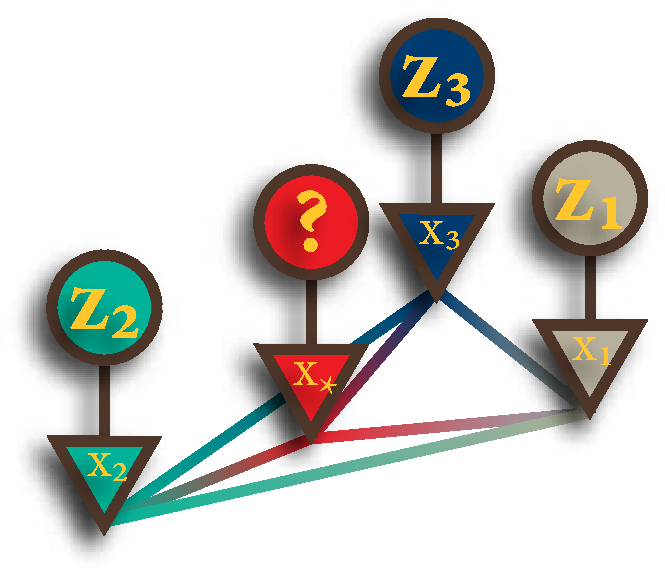
\includegraphics[width=\textwidth]{gp_inference_question}

\column{.58\textwidth}
Given some test value $x_*$, we now have:
\begin{align*}
\begin{bmatrix} z_1 \\ z_2 \\ z_3 \\ \textcolor{red}{?} \end{bmatrix} 
& \sim \N\left(\begin{bmatrix} 0 \\ 0 \\ 0 \\ \textcolor{red}{0} \end{bmatrix}, \begin{bmatrix} \tilde k_{11} & k_{12} & k_{13} & \textcolor{red}{k_{1*}} \\ k_{21} & \tilde k_{22} & k_{23} & \textcolor{red}{k_{2*}} \\ k_{31} & k_{32} & \tilde k_{33} &  \textcolor{red}{k_{3*}} \\ \textcolor{red}{k_{*1}} & \textcolor{red}{k_{*2}} & \textcolor{red}{k_{*3}} &  \textcolor{red}{k_{**}} \end{bmatrix} \right)
\end{align*}

where $\tilde k_{ii} = k_{ii} + \sigma^2$ to account for noisy observations.

\end{columns}

\end{frame}

%%%%%%%%%%%%%%%%%%%%%%%%%%%%%%%%%%%%%%%%%%%%%%%%%
\begin{frame}{Gaussian Process Inference II}
\Large

\begin{columns}[T] % align columns
\column{.38\textwidth}
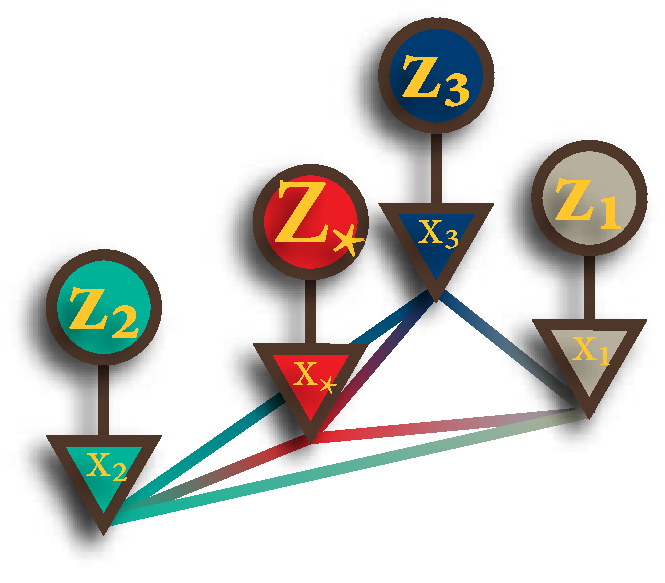
\includegraphics[width=\textwidth]{gp_inference}

\column{.58\textwidth}
Given some test value $x_*$, we now have:
\begin{align*}
\begin{bmatrix} \top \\ z \\ \bot \\ \textcolor{red}{Z_*} \end{bmatrix} 
& \sim \N\left(\begin{bmatrix} \top \\ 0 \\ \bot \\ \textcolor{red}{0} \end{bmatrix}, \begin{bmatrix} \ulcorner &  & \urcorner & \textcolor{red}{\top} \\  \multicolumn{3}{c}{K+\sigma^2 I}   & \textcolor{red}{k_*} \\ \llcorner &  & \lrcorner &  \textcolor{red}{\bot} \\ \textcolor{red}{\vdash} & \textcolor{red}{k_{*}^\tr} & \textcolor{red}{\dashv} &  \textcolor{red}{k_{**}} \end{bmatrix} \right)
\end{align*}
\end{columns}
It follows that:
\[
Z_*|\{X_*=x_*, \mathcal{D}\}
\sim \N(k_*^\intercal (K+\sigma^2I)^{-1} z, k_{**} - k_*^\intercal (K+\sigma^2I)^{-1} k_*))
\]

\end{frame}

%%%%%%%%%%%%%%%%%%%%%%%%%%%%%%%%%%%%%%%%%%%%%%%%%
\begin{frame}{Bernstein{\textendash}von Mises Theorem: Formal Statement}

\emph{Let the experiment $(P_\theta:\theta\in\Theta)$ be differentiable in quadratic mean at $\theta_0$ with nonsingular Fisher information matrix $I_{\theta_0}$, and suppose that for every $\epsilon>0$ there exists a sequence of tests $\phi_n$ such that:}
\[
P_{\theta_0}^n\phi_n \to 0, \quad
\sup_{\norm{\theta-\theta_0}\ge\epsilon} P_\theta^n(1-\phi_n) \to 0
\]
\emph{Furthermore, let the prior measure be absolutely continuous in a neighborhood of $\theta_0$ with a continuous positive density at $\theta_0$.  Then the corresponding posterior distributions satisfy}
\[
\norm{P_{\sqrt{n}(\bar\Theta_n-\theta_0)|X_1,\dotsc,X_n} - \N(\Delta_{n,\theta_0},I_{\theta_0}^{-1})}\xrightarrow{P_{\theta_0}^n} 0
\]
\emph{where $\Delta_{n,\theta_0}=\tfrac{1}{\sqrt{n}}\textstyle \sum_{i=1}^n I_{\theta_0}^{-1} \dot{\ell}_{\theta_0}(X_i)$, $\dot{\ell}_{\theta_0}$ is the score function of the model, and the norm is that of total variation.}

\footnotetext{see \cite{vdV98}}
\end{frame}

%%%%%%%%%%%%%%%%%%%%%%%%%%%%%%%%%%%%%%%%%%%%%%%%%
\begin{frame}{Bernstein{\textendash}von Mises Theorem: A Rephrasing}

\emph{Total variation is invariant to location and scale changes, so that}
\[
\norm{P_{\bar\Theta | X_1,\dotsc,X_n} - \N(\hat\theta_n, \tfrac{1}{n} I_\theta^{-1})}\xrightarrow{P_\theta^n} 0
\]

For a random variable $\Theta$, if we are given a sequence $X_1,X_2,\dotsc$ of random variables that each tell us a little bit more about $\Theta$, then $\bar\Theta | X_1,\dotsc,X_n$ converges in a very strong sense to a Gaussian with mean $\hat\theta_n$.
\footnotetext{see \cite{vdV98}}
\end{frame}

%%%%%%%%%%%%%%%%%%%%%%%%%%%%%%%%%%%%%%%%%%%%%%%%%
\begin{frame}{BrainGate setup}
\vspace{-25pt}
\begin{columns}
\column[t]{0.38\textwidth}
\begin{figure}
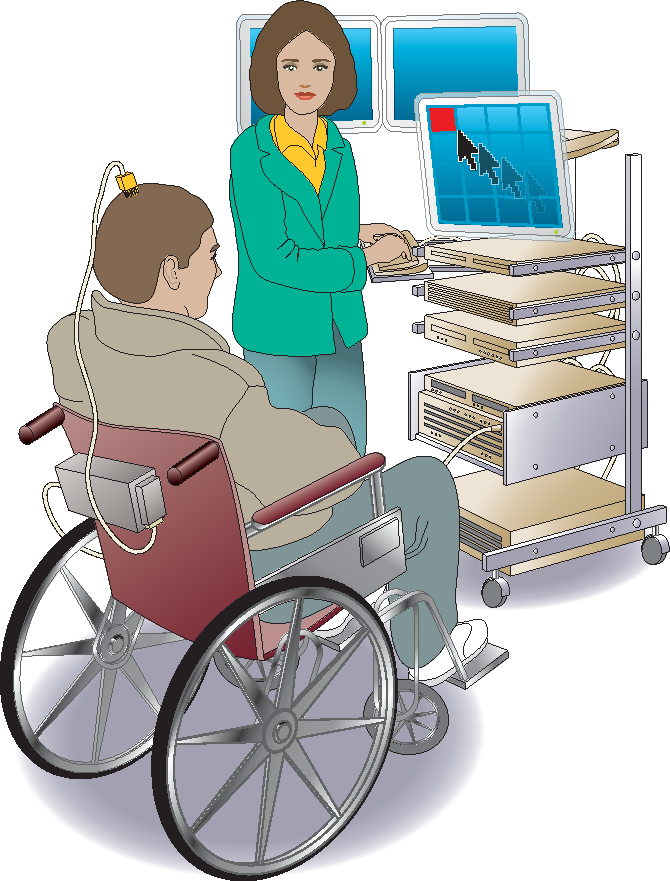
\includegraphics[width=\textwidth]{bg_setup_diagram}
\end{figure}
\column[t]{0.58\textwidth}
\begin{itemize}
\item BG uses the NeuroPort System (Blackrock Microsystems, Salt Lake City, UT) to sample raw neural signals for each electrode (30kHz) \\
\item an xPC target real-time operating system (Mathworks, Natick, MA) then processes these signals \\
\item signals are downsampled to 15kHz \& de-noised by subtracting an instantaneous common average reference using 40 of the 96 channels on each array with the lowest RMS value
\item de-noised signals were band-pass filtered between 250 Hz and 5000 Hz using an 8th order non-causal Butterworth filter
\item features are binned in 20ms non-overlapping increments
\end{itemize}
\end{columns}

\footnotetext{image credit: BrainGate; for more details, see dissertation section on ``Signal acquisition''}
\end{frame}

%%%%%%%%%%%%%%%%%%%%%%%%%%%%%%%%%%%%%%%%%%%%%%%%%
\begin{frame}{Challenges to Effective Decoding}
\Large
\begin{columns}
\column{0.58\textwidth}
\begin{itemize}
    \item good offline filters do not necessarily make good closed-loop filters~\cite{Jar13}
    \item metrics for BCI performance are non-standardized / lack of ground truth~\cite{Bil13,Tho14}
    \item the relationship between neural signals and intention changes over time~\cite{Per13,Per14}
\end{itemize}
\column{0.38\textwidth}
\begin{figure}
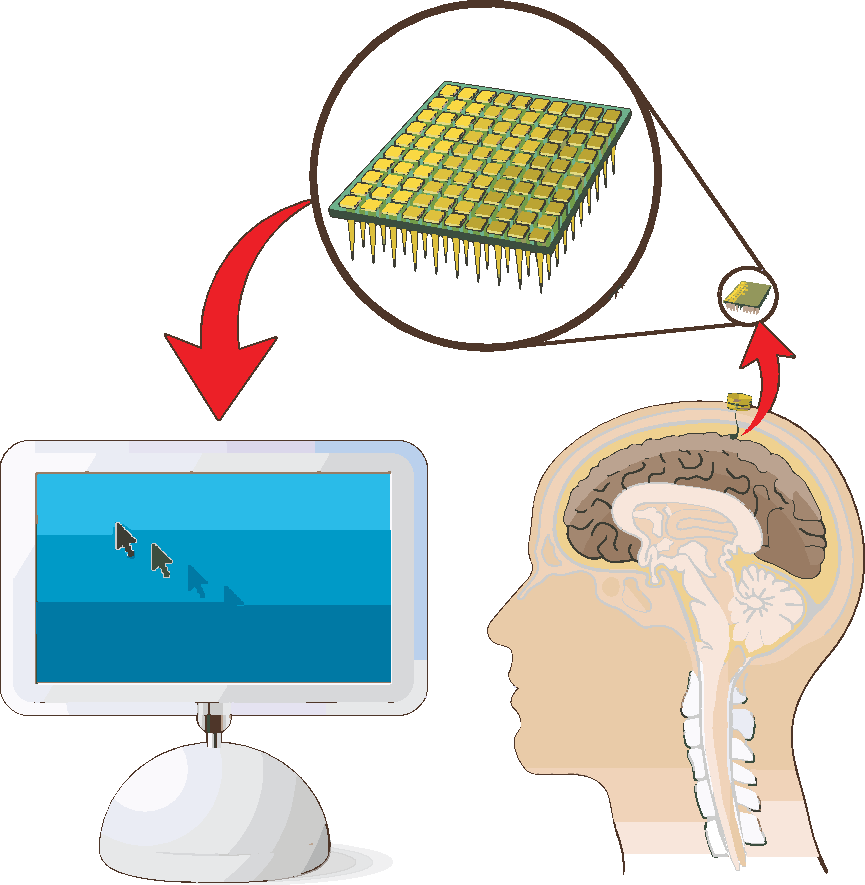
\includegraphics[width=\textwidth]{bg_diagram}
\end{figure}
\end{columns}

\footnotetext{image credit: BrainGate}
\end{frame}

%%%%%%%%%%%%%%%%%%%%%%%%%%%%%%%%%%%%%%%%%%%%%%%%%
\begin{frame}{BrainGate Calibration}
\begin{columns}
\column{0.58\textwidth}
\begin{enumerate}
    \item In the first 2-3 minutes, the computer moves the cursor and the participant imagines directing it (``open--loop'').
    \item In the next $\sim$ 10 minutes, the participant controls the cursor with assistance (error attenuation) that helps guide the cursor to the target (``closed--loop with error attenuation'').  With sequential retraining, the quality of data improves and the need for assistance decreases.
    \item Finally, the assistance is turned off completely and the participant assumes full control over the cursor.
    \end{enumerate}
\column{0.38\textwidth}
\begin{figure}
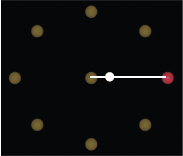
\includegraphics[width=0.5\textwidth]{bg_calibration1}
\caption{1. open--loop calibration}
\end{figure}
\begin{figure}
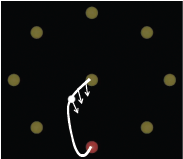
\includegraphics[width=0.5\textwidth]{bg_calibration2}
\caption{2. error attenuation}
\end{figure}
\end{columns}
\end{frame}

%%%%%%%%%%%%%%%%%%%%%%%%%%%%%%%%%%%%%%%%%%%%%%%%%
\begin{frame}{DKF implementation in Matlab: highlights}
\begin{figure}
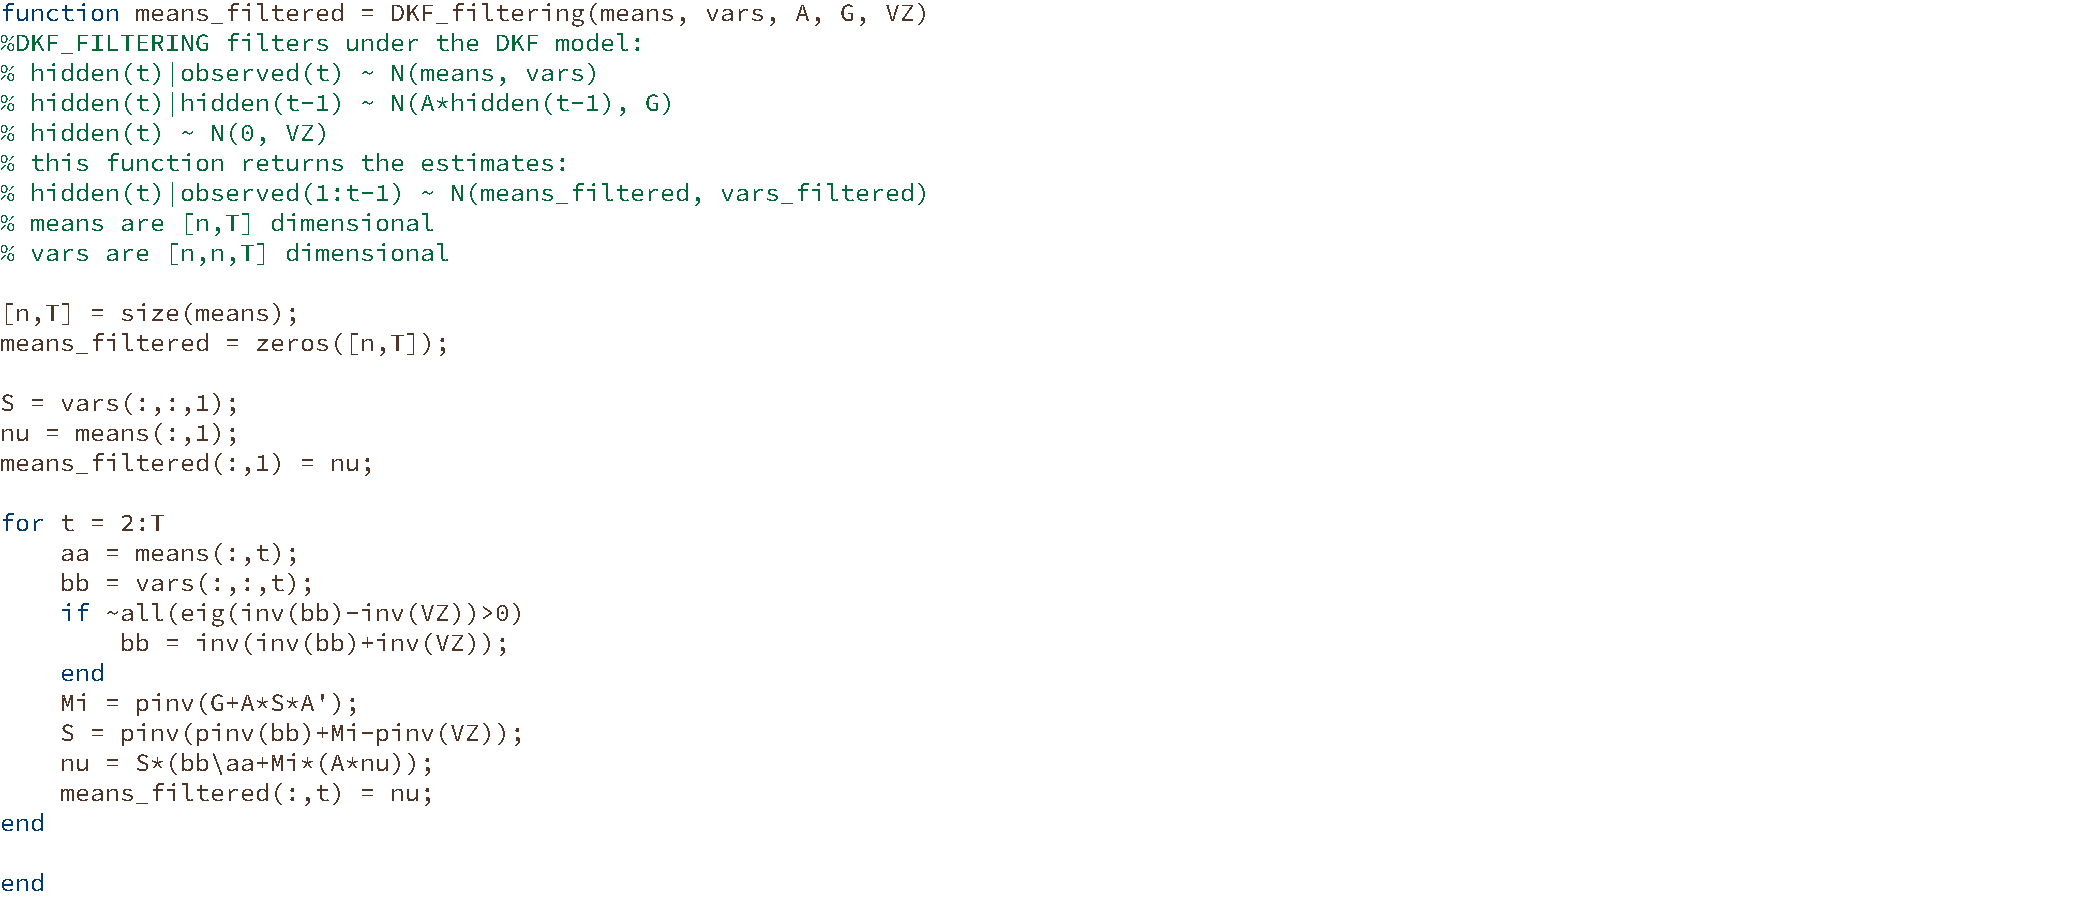
\includegraphics[width=\textwidth]{dkf-matlab}
\end{figure}
\end{frame}

%%%%%%%%%%%%%%%%%%%%%%%%%%%%%%%%%%%%%%%%%%%%%%%%%
\begin{frame}{Data Augmentation for Robustness}
\Large
\begin{enumerate}
    \item Take a datapoint:
    \begin{figure}
        
\includegraphics[height=0.03\textwidth]{data_aug1}
    \end{figure}
    \item Add noisy examples for neuron 1, with same label:
    \begin{figure}
        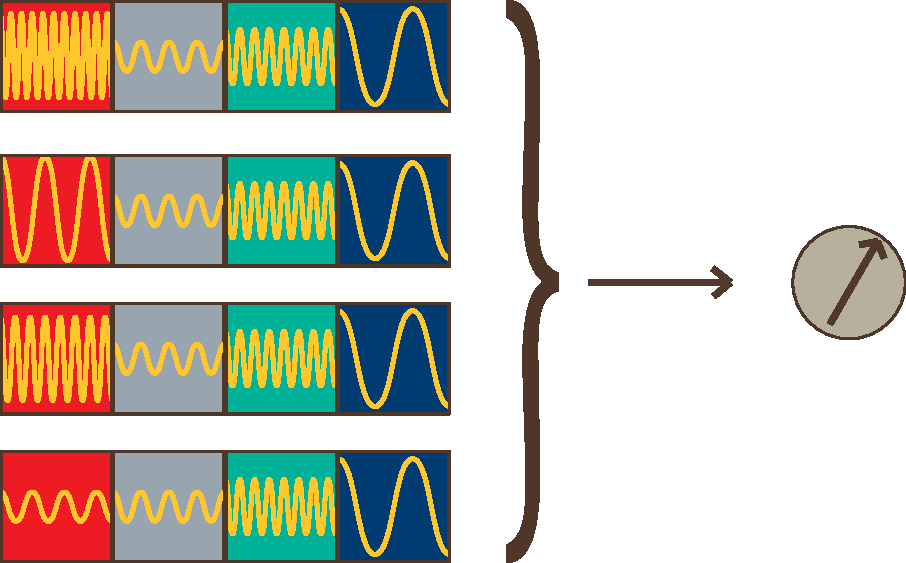
\includegraphics[height=0.1\textwidth]{data_aug2}
    \end{figure}
    \item Repeat this process for all other neurons:
    \begin{figure}
        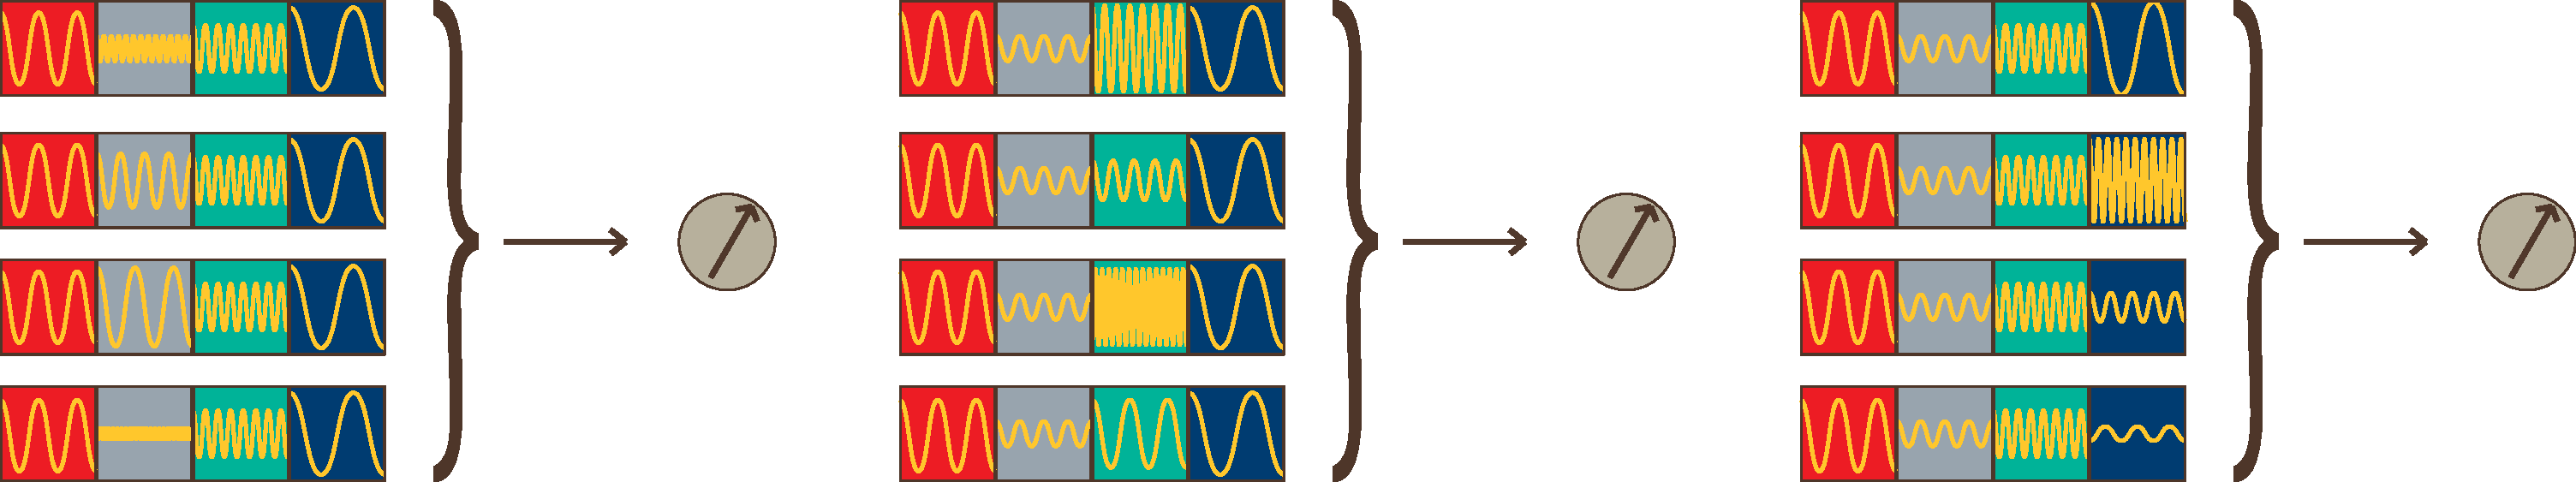
\includegraphics[height=0.1\textwidth]{data_aug3}
    \end{figure}
    \item Add all these new examples to your training set
\end{enumerate}

\end{frame}

%%%%%%%%%%%%%%%%%%%%%%%%%%%%%%%%%%%%%%%%%%%%%%%%%
\begin{frame}[allowframebreaks]
  \frametitle{References}
  \printbibliography
\end{frame}

\end{document}
